\documentclass[11pt,a4paper,twoside,english,svgnames]{report}
\usepackage[utf8]{inputenc} % force the use of utf8
\usepackage[T1]{fontenc} % font encoding, allows accents (T1 font encoding is an 8-bit encoding)
\usepackage[autostyle, english = american]{csquotes} % auto replacement of quotes
\MakeOuterQuote{"}
\usepackage[top=3.2cm,bottom=3.2cm,outer=2.7cm,inner=3.7cm]{geometry} % http://tex.stackexchange.com/questions/62311/a4paper-where-should-i-declare-it-in-document-class-or-geometry // another option: papersize={21cm,29.7cm}
\usepackage[english]{babel} % translate everything in the desired language: table of contents, etc. 'english' can be replaced with 'francais'
\usepackage[toc,page,header]{appendix} % cool appendices
\usepackage{graphicx} % images management
\usepackage{wrapfig} % floating images
\usepackage[format=plain,labelfont=bf,font=small,justification=centering,margin=10pt]{caption} % allow multiline captions in figures,
\usepackage{float} % allow \begin{figure}[H] and \begin{table}[H] (to really force positionning, unlike h!)
\usepackage{array} % allow arrays
\usepackage[super]{nth} % allow to write \nth(1) to write 1st, etc
\usepackage{fancyhdr} % headers/footers management (overrides empty, plain and headings)
\usepackage{upquote} % without this, lslisting replace vertical singles quotes with curved ones
\usepackage{listings} % code insertion (MUST BE WRITTEN AFTER BABEL)
\usepackage[
            backend=biber,
            style=numeric,
            sorting=none, % nty = name title year
            url=true, % always show url when provided
            ]{biblatex}
\addbibresource{bibliography.bib} % can be written only here in the preambule
\usepackage[nottoc,notlot,notlof]{tocbibind} % add the bibliography to the ToC ; nottoc,notlot,notlof remove the ToC, List of Tables and List of Figures from the ToC
%\usepackage{pdfpages} % include PDF documents
\usepackage{enumitem} % for /setlist
\usepackage{color,soul} % add some colors and hightlight
\usepackage{xcolor} % more colors
\usepackage{afterpage} % allow to execute command after the current page ends
\usepackage[hidelinks,
            colorlinks  = false, % no borders, colors enabled
            anchorcolor = blue,
            linkcolor   = black, % links in table of contents
            urlcolor    = blue,
            citecolor   = blue,
            breaklinks  = true]{hyperref}
\newcommand{\MYhref}[3][blue]{\href{#2}{\color{#1}{#3}}}%
\usepackage[%nonumberlist, % if enabled, suppress the index (entry locations)
            toc,% displayed in toc
            numberedsection,% displayed as a numbered section in toc
            xindy]{glossaries} % glossary without page numbers (references), with a number in the toc, with xindy style. MUST BE WRITTEN AFTER HYPERREF
\renewcommand{\glsglossarymark}[1]{} % Prevent 'glossaries' from changing the header (took here: http://mirror.ox.ac.uk/sites/ctan.org/macros/latex/contrib/glossaries/glossaries-user.pdf)

% List settings
\setlist{itemsep=.5em}
\setlist[itemize,2]{label={$\bullet$}} % use bullets for nested itemize in level 2

% Glossary settings
\setglossarystyle{listgroup}
\loadglsentries{glossary.tex}
\makeglossaries

% REQUIRES
% Nothing

% Transform \listoffigures and \listoftables into \section* instead of \chapter*
% Original "/usr/share/texlive/texmf-dist/tex/latex/base/report.cls" edited
\makeatletter
  \renewcommand\listoffigures{%
      \if@twocolumn
        \@restonecoltrue\onecolumn
      \else
        \@restonecolfalse
      \fi
      \section*{\listfigurename}% edited
        % \@mkboth{\MakeUppercase\listfigurename}%
        %         {\MakeUppercase\listfigurename}%
      \@starttoc{lof}%
      \if@restonecol\twocolumn\fi
      }
  % \newcommand*\l@figure{\@dottedtocline{1}{1.5em}{2.3em}}
  \renewcommand\listoftables{%
      \if@twocolumn
        \@restonecoltrue\onecolumn
      \else
        \@restonecolfalse
      \fi
      \section*{\listtablename}% edited
        % \@mkboth{%
        %     \MakeUppercase\listtablename}%
        %    {\MakeUppercase\listtablename}%
      \@starttoc{lot}%
      \if@restonecol\twocolumn\fi
      }
\makeatother
% REQUIRE
% \usepackage{color}
% \usepackage{listings} % (MUST BE WRITTEN AFTER BABEL)

% General colors
\definecolor{comment}{rgb}{0.12, 0.38, 0.18 } % adjusted, in Eclipse: {0.25, 0.42, 0.30 } = #3F6A4D
\definecolor{keyword}{rgb}{0.2, 0.2, 0.8} 
\definecolor{string}{rgb}{0.06, 0.10, 0.98} % #101AF9

% Language-specific colors
% JavaScript
\definecolor{darkgray}{rgb}{.4,.4,.4}
%\definecolor{purple}{rgb}{0.65, 0.12, 0.82}

% % hack to force UTF-8 compatibility (for french only)
% \lstset{
%         extendedchars=true,
%         literate={à}{{\`a}}1 {â}{{\^a}}1 %                         lettre a
%                  {À}{{\`A}}1 {Â}{{\^A}}1 %                         lettre A
%                  {ç}{{\c{c}}}1 %                                   lettre c
%                  {Ç}{{\c{C}}}1 %                                   lettre C
%                  {é}{{\'e}}1 {è}{{\`e}}1 {ê}{{\^e}}1 {ë}{{\"e}}1 % lettre e
%                  {É}{{\'E}}1 {È}{{\`E}}1 {Ê}{{\^E}}1 {Ë}{{\"E}}1 % lettre E
%                  {î}{{\^i}}1 {ï}{{\"i}}1 %                         lettre i
%                  {Î}{{\^I}}1 {Ï}{{\"I}}1 %                         lettre I
%                  {ô}{{\^o}}1 %                                     lettre o
%                  {Ô}{{\^O}}1 %                                     lettre O
%                  {œ}{{\oe}}1 %                                     lettre oe
%                  {Œ}{{\OE}}1 %                                     lettre OE
%                  {ù}{{\`u}}1 {û}{{\^u}}1 {ü}{{\"u}}1 %             lettre u
%                  {Ù}{{\`U}}1 {Û}{{\^U}}1 {Ü}{{\"U}}1 %             lettre U
% }

% General rules
\lstset{
  rulecolor=\color{black!50},
  backgroundcolor = \color{blue!10},
  numbers=none, %left % display line numbers
  showspaces=false,
  showtabs=false,
  breaklines=true,
  showstringspaces=false,
  breakatwhitespace=false,
  commentstyle=\color{comment},
  keywordstyle=\color{keyword},
  stringstyle=\color{string},
  basicstyle=\ttfamily,
  extendedchars=true,
  emph=[2]{In},
  emphstyle=[2]\color{black!70},
  morecomment=[l][\color{blue}]{Out},
  frame=single,
  frameround=tttt,
  framerule=0.3pt,
  framesep=4pt,
  belowcaptionskip=2.1pt
}

% % Define "Javascript" because lstlistings doesn't know it
% Taken from https://gist.github.com/Geruhn/3d21f60a869457373d84
\lstdefinelanguage{javascript}{
  keywords={break, case, catch, continue, debugger, default, delete, do, else, false, finally, for, function, if, in, instanceof, new, null, return, switch, this, throw, true, try, typeof, var, void, while, with},
  morecomment=[l]{//},
  morecomment=[s]{/*}{*/},
  morestring=[b]',
  morestring=[b]",
  ndkeywords={class, export, boolean, throw, implements, import, this},
  %keywordstyle=\color{blue}\bfseries,
  ndkeywordstyle=\color{darkgray}\bfseries,
  identifierstyle=\color{black},
  %commentstyle=\color{purple}\ttfamily,
  %stringstyle=\color{red}\ttfamily,
  sensitive=true
}

% Usage: \javascript
\newcommand{\javascript}{\lstset{
  language=javascript,
  title={{\setlength{\fboxsep}{1pt}\fcolorbox{orange}{yellow!20}{\sffamily\scriptsize
              \textcolor{gray!10}{\_}JavaScript\textcolor{gray!10}{\_}}}}
  }
}

% Usage: \code{My title}
\newcommand{\code}[1]{\lstset{
  language=,
  title={{\setlength{\fboxsep}{1pt}\fcolorbox{orange}{yellow!20}{\sffamily\scriptsize
              \textcolor{gray!10}{\_}{#1}\textcolor{gray!10}{\_}}}}
  }
}

% Usage: \sql
\newcommand{\sql}{\lstset{
  language=SQL,
  title={{\setlength{\fboxsep}{1pt}\fcolorbox{orange}{yellow!20}{\sffamily\scriptsize
              \textcolor{gray!10}{\_}SQL\textcolor{gray!10}{\_}}}}
  }
}

% Usage: \fakeshell
\newcommand{\fakeshell}{\lstset{
  language=bash
  }
}
% REQUIRES
% Nothing

% Redefine chapter titles: only display the title and remove useless blank space
% Original "/usr/share/texlive/texmf-dist/tex/latex/base/report.cls" edited
\makeatletter
  \def\@makechapterhead#1{% chapter{}
  \vspace*{0\p@}% 50 before
  {\parindent \z@ \raggedright \normalfont
    %\ifnum \c@secnumdepth >\m@ne
    %    \huge\bfseries \@chapapp\space \thechapter
    %    \par\nobreak
    %    \vskip 20\p@
    %\fi
    \interlinepenalty\@M
    \Huge \bfseries \thechapter\quad #1   
    \vskip 40\p@
  }}
  \def\@makeschapterhead#1{% chapter*{}
  \vspace*{0\p@}% 50 before
  {\parindent \z@ \raggedright
    \normalfont
    \interlinepenalty\@M
    \Huge \bfseries  #1\par\nobreak
    \vskip 40\p@
  }}
\makeatother
% REQUIRES
% \usepackage{fancyhdr} % headers/footers management (overrides empty, plain and headings)

% THE ORDER IS REALLY IMPORTANT, OTHERWISE IT WILL BREAK THINGS

% 1.
% Redefines the existing 'plain' style, (because 'chapter' and \tableofcontents ignores the page style currently in effect for their first page)
\fancypagestyle{plain}{
    % Took from: http://anorien.csc.warwick.ac.uk/mirrors/CTAN/macros/latex/contrib/fancyhdr/fancyhdr.pdf
    \fancyhead[LO,RE]{\slshape \leftmark}
    \fancyhead[LE,RO]{\slshape \rightmark}

    % Footers
    \renewcommand{\footrulewidth}{0.4pt}
    \fancyfoot[C]{The Smiths -- TN09 -- Romain \textsc{Pellerin}}
    \fancyfoot[LE,RO]{\ifdefined\thepage \thepage \fi} % to be used with \pagenumbering{gobble} % no numerotation
    % \fancyfoot[LE,RO]{\ifnum\thepage>0 \thepage \fi} % to be used with %\addtocounter{page}{-4} % numerotation begins at 1 + (-4)
}

% 2.
\pagestyle{plain}

% 3.
% http://tex.stackexchange.com/questions/111223/markboth-is-not-working-when-using-chapter-and-section
% Took from : http://ftp.snt.utwente.nl/pub/software/tex/macros/latex/contrib/fancyhdr/fancyhdr.pdf
\renewcommand{\chaptermark}[1]{\markboth{}{\MakeUppercase{\thechapter.\ #1}}}
\renewcommand{\sectionmark}[1]{}

% NORMALLY
% \renewcommand{\chaptermark}[1]{\markboth{\MakeUppercase{\thechapter.\ #1}}{}}
% \renewcommand{\sectionmark}[1]{\markright{\thesection.\ #1}} % To be edited to change the header and footer

\title{Internship report}
\author{Romain PELLERIN}
\date\today
\setcounter{tocdepth}{2} % ToC depth


\begin{document}
\pagenumbering{gobble} % no numeration, will start after the ToC
\nocite{*} % include everything that has not been mentionned, into the bibliography (PUT here to preserve the order of appearance), cause there are other commands \cite later

\thispagestyle{empty} % only applies to this page
\noindent
\includegraphics[height=2cm]{images/logo-smiths.png}\hfill
\includegraphics[height=2cm]{images/logo-utc.png}\\

\bigskip

\begin{center}
\vspace{3cm}

\noindent{\LARGE\MYhref[black]{http://www.utc.fr/}{Université de Technologie de Compiègne}}

\medskip

{\large Computer Science department (\textit{Génie Informatique})}

\vspace{3cm}
\noindent\fbox{
\begin{minipage}{.9\textwidth}
\begin{center}
    \vspace{0.3cm}\Large{\textbf{Internship report (TN09)}}\vspace{0.3cm}\\
    \vspace{0.3cm}\LARGE{\textbf{The Smiths}}\vspace{0.3cm}\\
    \vspace{0.1cm}\large{Amsterdam, the Netherlands}\vspace{0.3cm}\\
\end{center}
\end{minipage}}

\vspace{3cm}

\def\arraystretch{1.5} %  1 is the default // add '|' where you want vertical lines
\begin{tabular}{>{\hfill\arraybackslash}p{5cm}p{5cm}}
%\hline
    \multicolumn{2}{c}{\textbf{Romain \textsc{PELLERIN}}}\\\\
%\hline
    \multicolumn{2}{c}{\textbf{Mentor teacher:} Stéphane \textsc{MOTTELET}}\\
%\hline
     %Supervisor: & Wienke \textsc{GIEZEMAN}\\\\
     \multicolumn{2}{c}{\textbf{Supervisor:} Wienke \textsc{GIEZEMAN}}\\\\
%\hline
    \multicolumn{2}{c}{Autumn 2015 (A15)}\\
    %\multicolumn{2}{c}{\textit{from September 1, 2015 to February 12, 2016}}\\
%\hline

\end{tabular}
\vfill

{\footnotesize Last update: \today}
\end{center}
\newpage % starts a new page. Might contains floating images .
% \clearpage % starts a new page completely empty.
\thispagestyle{empty} % only applies to this page
~\\
\chapter*{\centering\vfill Acknowledgments}

This internship was, as expected, a great opportunity to discover a new country, the Netherlands, and to learn a lot. Therefore, I want to express my deepest gratitude to:

\bigskip

\textbf{Wienke \textsc{Giezeman}} for this internship offer and his warm welcoming within his startup. As a great entrepreneur and CEO, his positive attitude is a real strength. He perfectly knows how to motivate someone. He is a natural born leader, always pushing further everyone's limits.

\bigskip

\textbf{Pierre \textsc{Van de Velde}} for his everyday help, his kindness, and the confidence he had in me. His sense of leadership makes him an excellent CTO. His experience and guidance allowed me to learn a lot. A great ambitious guy playing a key role in the company.

\bigskip

\textbf{Matthias \textsc{Benkort}}, my friend, colleague and housemate. Always ready to help and share his knowledge, he is very skilled and extremely motivated. He is one of those people interested in everything. He truly is inspiring. He loves challenging himself everyday, which I greatly appreciated.

\bigskip

\textbf{Wessel \textsc{Versluis}}, our crazy designer (in a good way), for making life a big joke! He was the one bringing us joy, as soon as he would come in to the office. Nonetheless, he proved us to be highly competent. I will definitely miss him.

\bigskip

\textbf{All the people at Rockstart}. Without them, no crazy foosball matches, no tasty sandwiches and more importantly, no great coworkers!

\bigskip

\textbf{Stéphane \textsc{Mottelet}}, for his availability and help. He was the link between the UTC and myself, all along.

\bigskip

\textbf{Every person I had the chance to meet in Amsterdam} for making my life so beautiful for six months. Amsterdam is a great multicultural city, full of places to explore, things to see. Thank you, Amsterdamers.
\vfill

\thispagestyle{empty} % applyed to acknowledgments
\newpage % starts a new page. Might contains floating images .
% \clearpage % starts a new page completely empty.
\thispagestyle{empty} % only applies to this page
~\\

\tableofcontents

%%%%%%%%% FIGURES AND TABLES ON THE SAME PAGE %%%%%%%%%
\chapter*{Figures and Tables\markboth{\MakeUppercase{Figures and Tables}}{\MakeUppercase{Figures and Tables}}}
\listoffigures
\listoftables
\newpage % starts a new page. Might contains floating images .
% \clearpage % starts a new page completely empty.
\thispagestyle{empty} % only applies to this page
~\\

\cleardoublepage
\pagenumbering{arabic} % re-enable numering

\chapter*{Foreword}
\markboth{}{\MakeUppercase{Foreword}}
\addcontentsline{toc}{chapter}{Foreword}

In 2016, mobile applications are key in most commercial businesses. Everyone used to have a website in the early 2000's, now everyone needs to have a mobile application. As from 2007, the introduction of the iPhone by Apple, this industry has never stopped growing, unceasingly, following a steep curve.

\medskip

Nowadays, the market shares are pretty simple: Android (acquired in 2005 and now developed by Google) and iOS (created and developed by Apple, initially released in 2007) rule the world. Windows Phone (Microsoft) ranks third and Blackberry (formerly known as Research in Motion) is almost dead. Consequently, anyone who wants to be "mobile" has to be present on, at least, both Android and iOS app markets.

\medskip

Android's main programming language for developing apps is Java, whereas iOS uses Objective-C and Swift. Development for Android and iOS implies knowing both platforms, both SDKs, at least two languages, and quite often, it requires twice as much time as it would take for one operating system. As a result, some people had the idea to create "cross-platform" mobile SDKs. Most of these use web technologies such as HTML5 or JavaScript. Basically, "cross-platform", in this context, means enabling developers to build web apps, in addition to mobile applications, at the same time, from the same codebase. Among the most popular are \href{http://phonegap.com/}{PhoneGap} and \textbf{\href{http://www.appcelerator.com/}{Appcelerator Titanium}}.

\medskip

Back in June 2015, when I was offered an intern position at the Smiths, I saw that as a new challenge for me. I was quite unfamiliar to JavaScript, and even more with cross-platform development using JavaScript. As I had heard a lot of good things about that language and its increasing ubiquity, without any doubt, I signed.

\bigskip

\begin{itshape}
Furthermore, I would like to mention that, in the meantime, this internship offered me an opportunity to dive deeper into broad subjects about Computer Science. As a consequence, it allowed me to write about such topics on a personal blog, accessible at \href{http://blog.romainpellerin.eu/}{blog.romainpellerin.eu}. Some parts of these blog posts were reused in this internship report.
\end{itshape}

\section*{Technical summary}
\addcontentsline{toc}{section}{Technical summary}

Between PhoneGap and Titanium, The Smiths (my internship company) has decided to go with the latter. Why? Unlike PhoneGap, Titanium enables us to create "native applications". Fundamentally, every app developed with Titanium is made of two main components: the Titanium API, built in native code (Java or Objective-C) by Appcelerator, and JavaScript code (written by developers, like us), dynamically injected and evaluated at runtime by Titanium. Under the hoods, Titanium acts as a "bridge", a "proxy" between JavaScript and the platform. On the other hand, PhoneGap creates applications that run within the platform web browser. Applications developed with PhoneGap lack performance and are browser-limited. On the contrary, Titanium apps can access all the native functions and services offered by the system, as long as the company behind (here Appcelerator) keeps it up-to-date and integrates changes brought by newer versions. Regarding Titanium, they try to release new versions of Titanium frequently. And nearly every month, we get minor patches.

\medskip

During this first two months, I was assigned an entire new project: \textbf{Bearleaders}. My mission was to, first, write the specifications, working closely to our designer. Then, I had to develop a back-end (an API) (hosted on \href{http://www.parse.com}{Parse.com}), documenting it, with a back-office for the administrator -- our client. Finally, I was supposed to develop the Android and iOS applications using Titanium. Unfortunately, the project was abruptly canceled right before starting developing the apps, due to a poor relationship with our client. Since then, I had been working on an internal project, \textbf{KopenVerkopen}, which is the Dutch equivalent to \href{http://www.leboncoin.fr/}{leboncoin.fr}. I also helped on another project for a client from December to January.

\medskip

Another aspect of my mission involved carrying out research, especially about \textbf{APIs} and \textbf{Continuous Integration}. I have conducted a lot of searches about the former. As to the latter, with Matthias' help, we had been trying to set up an entire workflow, in order to add as much automation as possible. First, we "standardized" our Git workflow, then wrote many scripts and eventually came up with a well working solution. We also established a few rules to be followed by everyone in the company.

\medskip

Last but not least, during the first three months, I had been trying to get used to \textbf{functional programming} principles. I learnt a lot by using some libraries bringing functional programming into JavaScript, once again thanks to Matthias' involvement. The idea was to write code reusable in any context.

\bigskip

On many aspects, this internship was rich and full of lessons. It was the perfect chance to put my knowledge into practice and learn even further.
\chapter{Introduction}
\section{The Smiths}

The Smiths is a startup created in early 2015 in Amsterdam, by two people, Wienke \textsc{Giezeman}, a Dutch entrepreneur, and Pierre \textsc{Van De Velde}, a French developer, who is also a former employee of Wienke.

\subsection{Behind the scenes}

Back in 2012, Wienke created a first startup called WappZapp (a video-on-demand service provider for the Dutch public). He hired Pierre as an intern, in 2013.

\medskip

During 2014, while unceasingly growing at a regular pace, they changed their economic model, offering customers more services (basically, more content to watch) for a few euros. Then, they had been struggling for months, trying to convert all the users to that new freenium model, without success. Although the product was quite robust and this pricing strategy was supposed to work, it is always hard to convince customers, especially those used to free mobile apps. At this point, they just decided to stop there.

\medskip

Soon after, Wienke and Pierre got back to work, both of them owning their own little company (self-employment). Pierre had gained experience with Titanium, a cross-platform SDK\footnote{\textit{Software Development Kit}, a set of software development tools allowing the creation of applications (from software programs to hardware frameworks, video-games, and so on).} for mobile development, as it was the one they used for WappZapp. Quite naturally, they continued working with it: developing apps with Titanium for clients (companies or individuals), that is what they decided to do for a living. Wienke would be the CEO and responsible for finding clients whereas Pierre would be the CTO and developer. A few weeks later they were hiring Matthias as an intern. In solely a couple of weeks, \textbf{from the ashes of WappZapp was born The Smiths}.

\subsection{Who \& What}

At the moment, The Smiths is a sort of agency, "\textit{supplying companies with Titanium developers}" (that is their motto), with full expertise in mobile applications developed with Titanium.

\medskip

As I wrote above, in February 2015, they hired Matthias \textsc{Benkort}, a French student in Computer Science, as an intern. Six months later, he graduated. Then, they decided to offer him a full-time position, which he accepted. That happened approximately when I arrived, in late September 2015. Since the very beginning, they have also been working closely with a Dutch independent designer, still a student but also a freelancer in his spare time, Wessel \textsc{Versluis}. In the meantime, they also hired a remote developer from Vietnam, Nguyen \textsc{Bao Duy}, a freelancer, who would be working from time to time for the company.

\medskip

The goal of the company is pretty simple: they try to work half of the time on projects for clients (involving Titanium), in order to earn money and make a living (and pay interns, at the same time). On the other hand, the rest of the time is dedicated to internal projects with three main ideas in mind:

\begin{itemize}
  \item To gain experience in project management (finding a working workflow), try trendy technologies, and improve oneself on a regular basis (in functional programming for example)
  \item To contribute to the Titanium community, especially by developing open source modules and widgets
  \item To show what the company achieved to attract new clients, by developing internal projects
\end{itemize}

The long-term strategy is to progressively evolve, from a simple development agency to something bigger, adopting cutting-edge technologies such as React\footnote{A new and popular JavaScript framework developed and powered by Facebook, see \href{https://facebook.github.io/react/}{facebook.github.io/react/}}. They also want to explore new horizons, including machine-learning, artificial intelligence, or predictive analytics.

\subsection{The office}

\begin{figure}[H]
   \centering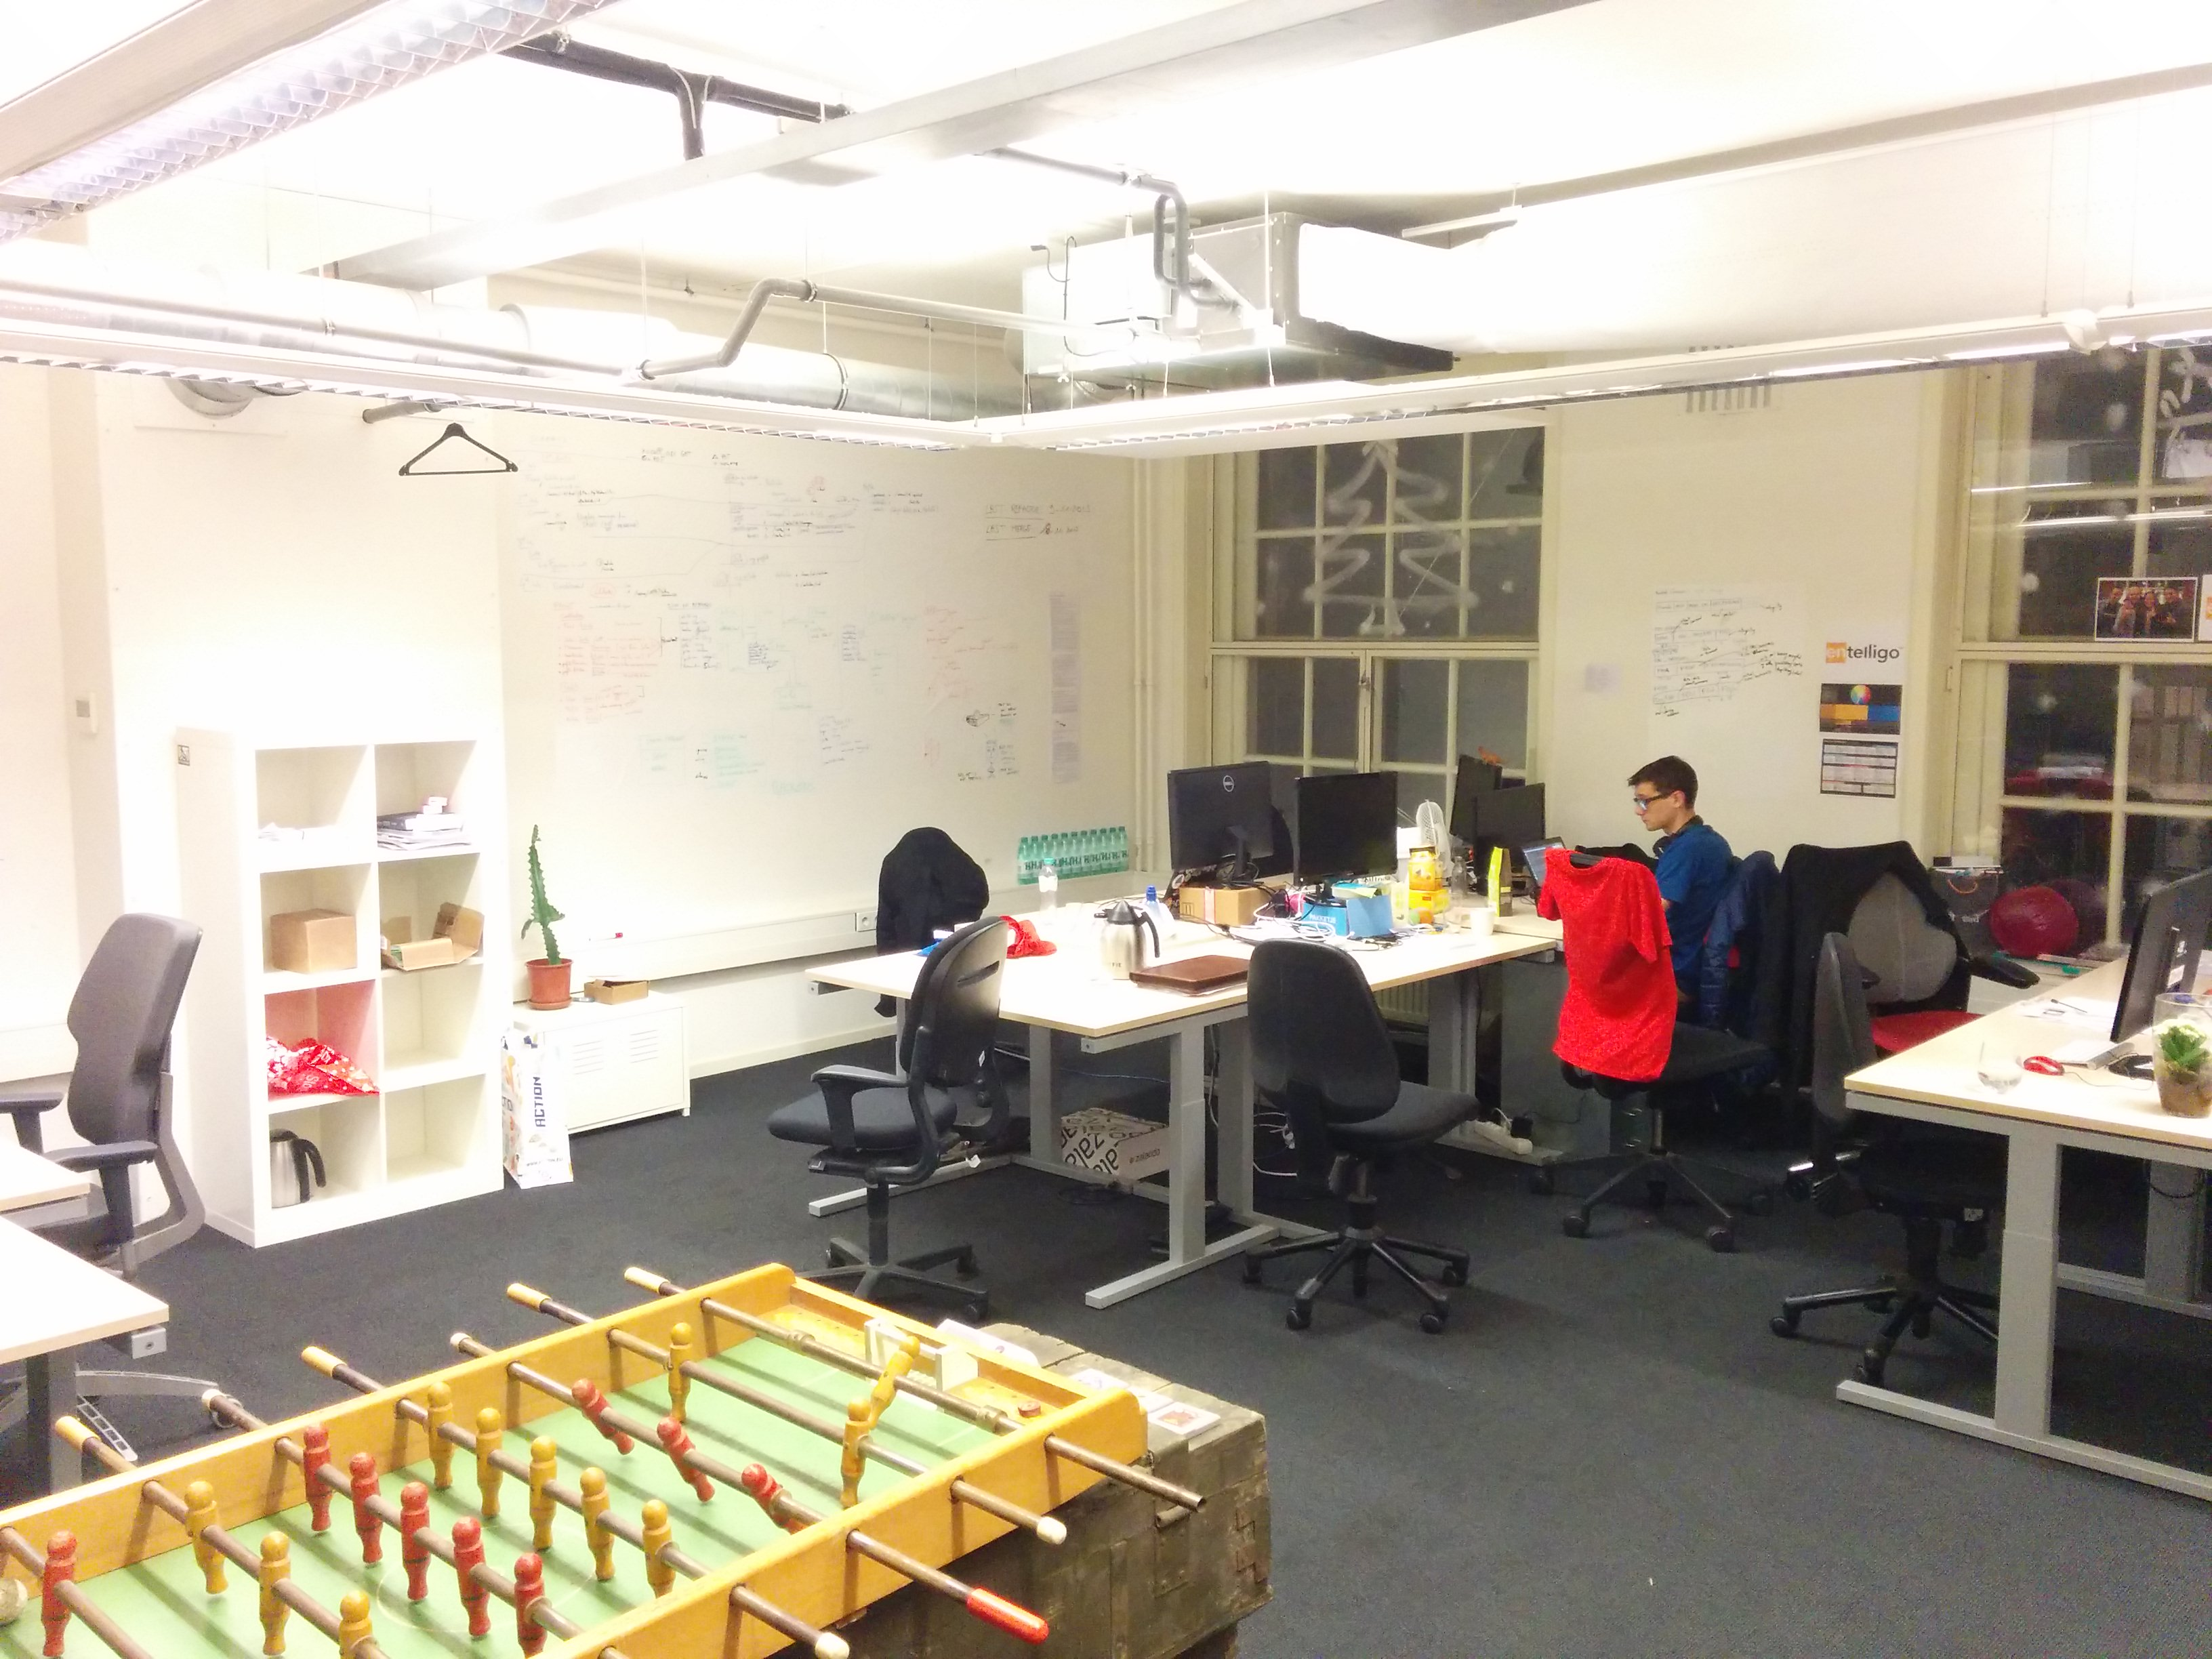
\includegraphics[width=0.75\textwidth]{images/office.jpg}
   \caption[Our office]{Our office}
\end{figure}

The Smiths has its office located at Herengracht 182, in Amsterdam. It is in the very city center, close to everything. We were in an incubator called \textbf{\href{http://www.rockstart.com/}{Rockstart}} whose mottos are "\textit{Step Forward. Start.}" and "\textit{We love startups}". Basically, they provide startups with as many desks as they need, in one of the four floors, with free coffee and tea. In parallel, they prepare everything for lunch at a reasonable price. Moreover, every startup can book a huge old ballroom for special events, most of the time for free.

\medskip

It is a very nice place for startups to prosper, so inspiring, full of young people, mostly developers. The atmosphere is really favorable to innovation, there is always someone challenging your ideas. What is more, we would often organize some crazy foosball competitions after lunch.

\subsection{Influence}

The Smiths has proven its clients a great ability to ship good mobile applications, highly scalable, and more importantly, with a good evolvability. Quite surprisingly, within a few months, The Smiths caught on with the Titanium community, thanks to a huge commitment.

\medskip

Every month, the Smiths were given the mission to organize the official Titanium meeting events. With an average of twenty attendees, there was usually three or four speakers, giving talks about mobile development with Titanium or any other related topic. The meetups were always sponsored by Appcelerator, the company behind Titanium, providing everyone with food and drinks.

\medskip

The company's commitment (and especially Matthias') to giving away open source modules, plugins or widgets allowed us to get praised sometimes.

\section{Titanium}

\begin{figure}[!h]
   \centering
\includegraphics[width=0.4\textwidth]{images/titanium.png}
   \caption{Titanium SDK}
\end{figure}

As I said earlier, everyone at the Smiths is dedicated to developing mobile applications with Titanium. So, let's dive into Titanium and look under the hood.

\subsection{Concept}

Titanium is an open-source framework\footnote{More or less a foundation, a structure or a platform for developers to build software programs. The code of a framework generally offers classes and functions that can be either reused of changed by user-written code. It is quite similar to an API (frameworks technically contains API(s)). "Framework" is a generic term that can basically define a lot for things.}/SDK, powered by Appcelerator, that allows developers to create and ship mobile apps very quickly, for both Android and iOS (and Windows Mobile), or create responsive web pages -- and all of this with the same codebase, written in JavaScript. It was firstly introduced in late 2008.

\medskip

Out of the box, Titanium does not impose nor recommend any particular project structure. The lack of best practices regarding project structures was, by the way, one of the biggest downsides in Titanium for years.

\medskip

However, since 2012, developers can also add a MVC-based\footnote{\textit{Model View Controller}, a popular architecture in software} framework on top of Titanium called Alloy, to bring a better architecture to their apps. It was designed to "\textit{rapidly develop quality Titanium applications}". To support the MVC architecture, the creators of Alloy also added \href{http://backbonejs.org/}{Backbone.js} and \href{http://underscorejs.org/}{Underscore.js}, which are JavaScript libraries, respectively providing Titanium with models (plus collections and events) and functional helpers.

\medskip

Basically, an accepted definition of working with Titanium could be

\begin{quote}
\textit{Simply write JavaScript code, Titanium will turn it into native code for each platform.}---Romain Pellerin
\end{quote}
In fact, not exactly. The JavaScript code is evaluated at runtime\footnote{When the mobile app is running}. Actually, what is in native code is the Titanium API\footnote{\textit{Application Programming Interface}, a set of routines, protocols and tools exposed to API consumers, to interact with a remote database or software for example. It is a level of abstraction.}, which acts as a "bridge" or "proxy" between our JavaScript code and the system calls (made in native code, depending on the platform, either in Java or Objective-C/Swift).

\subsection{Appcelerator}

Appcelerator is the company behind Titanium. Its core mission is obviously to support the development of Titanium, but not only. As Titanium is open-source, they mostly developed their business model thanks to other services. More and more, they tend to target enterprises instead of independent developers to generate revenue. As examples, their most successful products include real-time analytics, cloud services, and push notifications\footnote{For more information about their range of products, see \href{http://www.appcelerator.com/product/}{www.appcelerator.com/product/}}. They also provide their own IDE\footnote{\textit{Integrated Development Environment}, or more simply, a text editor linked to a compiler, with built-in tools like a linter, an embedded console, a source management system (Git or SVN, mainly), etc.} based on Eclipse, for free, as an alternative to the CLI\footnote{\textit{Command Line Interface}}.

\subsection{Alloy}

As exposed above, Appcelerator introduced in 2012 a new framework called Alloy. Basically, it is just a Titanium plugin (plugins will be quickly explained right below). This means that it is a piece of code run in the very first step of compilation. Briefly, what it brings are:

\begin{itemize}
  \item XML support to write and define views
  \item A new file format, \textbf{.tss}, a cousin of CSS, to declare styles and themes for views
  \item A new structure for Titanium projects, to better organize files under a relevant architecture
  \item A handful of global functions and variables aimed at easing simple tasks and objects storing, likewise a configuration file complementary to the original one provided by Titanium
  \item Two powerful JavaScript libraries: Backbone and Underscore (they respectively bring models and helpers)
\end{itemize}

Here is a new structure brought by Alloy, in the root directory \lstinline{app/}:

\begin{figure}[!h]
   \centering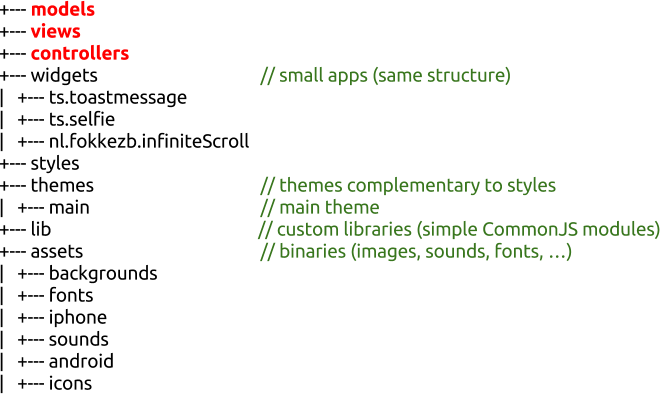
\includegraphics[width=0.8\textwidth]{images/Alloy.png}
   \caption[Alloy structure]{Alloy structure\\\textit{The widgets here are given as examples}}
\end{figure}

\subsubsection{How it works}

The way Alloy works is pretty simple and adds a lot of logic. There is a file at the root of \lstinline{app/}, called \lstinline{alloy.js}. It is the first file executed when the app is being launched. Then, Alloy runs the default controller located at \lstinline{controllers/index.js}. It also loads a default view if existing (\lstinline{views/index.js}) and it applies styles to that view (if existing as well, from \lstinline{styles/index.js} or from \lstinline{themes/}). Then, developers can start any other controller from an opened one, just by calling a built-in function of Alloy. The app will automatically try to launch the corresponding view and apply the corresponding styling (always according to the controller's name).

\subsection{Modules, widgets and plugins}

In spite of the fact that Titanium covers most of the native features available on both Android and iOS, it can not be 100\% up-to-date, considering new versions of Android and iOS are generally coming out once a year. Thus, they had to provide a way for developers to satisfy all their needs regarding cutting-edge features. Consequently, they "invented" modules.\\
Modules are one of the many strengths of Titanium. Modules are mostly written in native code (either Java for Android or Objective-C for iOS). They allow developers to add missing features to Titanium. Just like the official Titanium API, modules offer missing JavaScript APIs to Titanium developers. Many are available on the Web, either created by Appcelerator or independent developers.\\
For example, at some point I was looking for a way to add in-app purchases in an app. On Android, this feature is provided by the Google Services, which are not part of core Android -- it is a third-party app. Consequently, Titanium cannot bring it either, as it might be updated at any time by Google, and is not correlated to Android itself. In such a situation, modules are what I needed.

\medskip

On the other hand, widgets are small pieces of JavaScript code whose purpose is to add reusable components to an app, such as views, specific models or mere convenient functions. In simple words, one could see widgets as a Titanium app taken apart into smaller bits. Those bits can be made reusable, and then shared on the Web among the Titanium community. This way, one does not have to reinvent the wheel and can reuse other people's work. Widgets are brought by Alloy and have their own views, controllers, styles and assets.\\
As examples, there are widgets that bring helpers for API calls, some others bring views (a chat view for instance, with the input field and the list of messages), and so forth.\\
Widgets are much simpler pieces of code than modules and only written in JavaScript (and XML/TSS if they add view(s) and styling to them). They are minimalist Titanium apps with roughly the same file structure.

\medskip

Finally, Titanium also support plugins. Alloy is a concrete example of a plugin. I will not explain any further but in short, it is code being executed at the beginning of the compilation. Matthias, my colleague, created a plugin that transpiled\footnote{Transpiling is "taking source code written in one language and transforming into another language that has a similar level of abstraction". Source: \href{https://www.stevefenton.co.uk/2012/11/compiling-vs-transpiling/}{www.stevefenton.co.uk/2012/11/compiling-vs-transpiling/}} code written in ES6\footnote{ECMAScript 6, a.k.a ECMAScript 2015, is the latest JavaScript Specification, still not supported by Titanium and most web browsers} into ES5 thanks to Babel (a compiler whose only job is to transpile ES6 code into ES5). That process was automatically run right before the compilation, thanks to some tuning made with Titanium. He made it available\footnote{\href{https://www.npmjs.com/package/ti.es6}{www.npmjs.com/package/ti.es6}} to everyone and encountered a quite huge success quickly.

\subsection{Motivation to use Titanium}

Quite simply, the Smiths already had experience with Titanium in their previous startup (WappZapp). They could have decided to get back to native development or try another cross-platform tool but instead they decided to keep on with Titanium. Why? Merely because it is a robust SDK quite reliable, under intense development with an increasing community. Furthermore, it would allow the company to save money (one JavaScript developer is more easily findable and often cheaper than either a developer able to develop on both Android and iOS, or two distinct developers).

\section{My mission}

When I accepted the internship offer, in late Spring 2015, I got assigned one particular mission. The Smiths had just come to an agreement with a client for a new project and I would be responsible for the whole project, from the specifications to delivering the final product.

\medskip

After this first mission (abruptly aborted, but that will come later), I was reoriented to an internal project called KopenVerkopen, which is an app for selling items (like eBay). I also worked on another project for a different client, mostly in January 2016. For these purposes, I had to develop some Titanium widgets that the Smiths would reuse later.

\medskip

Aside my main missions, I have been trying to design a robust and efficient workflow. By workflow, I mean a tested and approved process for developing a software project. From the source code management, to shipping the product, including some automation, automated testing, and so on.\\
In the meantime, I also worked on APIs, trying to define a standard we would follow for each project, simple to use, evolvable and which takes advantage of all the strengths of the protocol HTTP.\\
Those two aside topics (APIs and workflow) will be treated in the next chapters to ease the overall understanding of this report. Then, the three projects will come in the remaining chapters.
\chapter[Continuous Integration]{Establishing an efficient workflow for software projects: Continuous Integration}

After having experienced software development in many languages, from desktop programs to mobile applications and web sites, comes a moment when I felt compelled to standardize my software development process. With Matthias' experience, we tried to define The Smiths' workflow more formally, even though they already had something that had been working for a little while.

\medskip

Our main concern was \textbf{continuous integration}. How to properly "synchronize" a team made of many developers, "spread all around the world", in different time zones? Indeed, as I said we were working with a developer from Vietnam. How to make sure there is no bottleneck at any level, during the development? First, let's have a look at the definition.

\medskip

\noindent What is \textbf{continuous integration}? According to Wikipedia, it is:

\begin{quote}
\textit{[...] the practice, in software engineering, of merging all developer working copies to a shared mainline several times a day.}
\end{quote}
But not only. It is much more than this. Let's dive into continuous integration.

\section{Purpose}

Continuous integration is an entire concept that tries to ease software development by making things much easier and flexible. Like agile methodology, it has been getting more and more popular since the beginning of the 2000's. Nowadays, it tends to be widely adopted in any kind of software company.

\subsection{Effortless automation}

Continuous integration is mostly about automation. By this, I mean being able to deploy flawlessly, many times a day. The documentation generation, testing and deploying have to become a commodity. Repetitive tasks are most of the time painful and should be performed by computers.

\subsection{Continuous testing}

\textbf{Every new release has to be tested}. Automatically. Without any human intervention. In a safe and minimal environment, not a human's environment with tons of programs, custom environment variables, outdated dependencies, etc. It is a human job to design the tests but running and validating them is a machine job. This way, the results can be shared with an entire team over automatic emails and archived.

\subsection{Documentation}

Writing documentation is for humans. Generating it is for machines. Again, it is a repetitive task that no one should be assigned. It is a waste of time. Machines can do it instead of us, at the right time, usually when a new release is about to come out. Furthermore, machines do not forget to bump the version numbers.

\subsection{Deploying}

With continuous integration, deploying should be as simple as a \lstinline{git push}. When time has come for deployment, no one should have to use \lstinline{ssh} or \lstinline{rcp}, not even \lstinline{ftp}. \textbf{It is unsafe insofar as it is too much of a risk to let a human get inside a production machine.} A developer has nothing to do in a production machine, as long as all the tests have been passed before pushing to production. All one can do is breaking something. A production machine is meant to be administrated by a sysadmin, no one else. Once it is set up, the only action required by developers is pushing code when it is ready to go live.

\medskip

It is the same story for releases. Packaging and releasing a new version must be a simple task anyone can do, not only the CTO, regardless of the OS, configuration, and so on.

\bigskip
\bigskip

\textbf{That is my point of view about Continuous Integration}, and it is shared by many developers. In fact, continuous integration should simply be regarded as an entire development workflow. It enables a team of developers (or even a single developer) to be more agile. You can easily get rid of god-awful tasks without actually deleting them, just by delegating them to computers. In parallel, it enables developers to improve maintainability and evolvability of the software they produce by adopting the right versioning and bug tracking tools.

\section{Deep diving into continuous integration}

At The Smiths, we identified \textbf{four main components} that we wanted as \textbf{core parts} of \textbf{our Continuous Integration process}:
\begin{itemize}
  \item Semantic versioning
  \item A Git workflow
  \item \href{https://travis-ci.com/}{Travis-ci.org}
  \item Agile methodology
\end{itemize}

\subsection{Semantic versioning}\label{semantic-versioning}

We decided to stick to the very simple rules proposed by \href{http://semver.org/}{semver.org}. Basically, it says that a version number should be something like \textsc{MAJOR.MINOR.PATCH}, where (what follows has been extracted from their website):
\begin{enumerate}
  \item \textsc{MAJOR} version when you make incompatible API changes
  \item \textsc{MINOR} version when you add functionality in a backwards-compatible manner
  \item \textsc{PATCH} version when you make backwards-compatible bug fixes
\end{enumerate}

Sticking to this rule forced us to think more about the logic behind the versions, reshape road maps more precisely, and allowed us to bump our version numbers more cleverly. We applied this to our mobile apps and Titanium widgets, bumping version numbers carefully over time.

\subsection{A successful Git workflow}

This part is clearly the most important, as it is being used every single day by everyone. In general, it is likely the most important aspect about continuous integration, to which we had paid a lot of attention.

\medskip

After some research, we came across a very popular Git workflow, the branching model\footnote{\href{http://nvie.com/posts/a-successful-git-branching-model/}{http://nvie.com/posts/a-successful-git-branching-model/}}. Please refer to the Appendix \ref{appendix-git} for a detailed diagram.

\medskip

Overall, it is the best Git workflow we have ever encountered. \textbf{So we adopted it, with some specificities: we made a few minor changes to that original branching workflow, in order to better suit our needs.} It can be applied to any kind of software project. I also need to mention that we use GitHub, the most famous web-based Git repository hosting service, because it offers some great features, such as Pull requests\footnote{A feature allowing anyone to submit code changes to a project, from a cloned repository, to the original one}, a bug tracker (issues), etc. Moreover, as most of our code has been open sourced (except our clients' core apps), it is not a problem at all. By the way, it also gives us a greater visibility, it is like giving away our widgets to the Titanium community thanks to GitHub.

\subsubsection{Our daily Git workflow at The Smiths}

\begin{itemize}
  \item There is a remote repository called \lstinline{origin}. It is owned by an organization created on GitHub called "TheSmiths", which gathers all of us. Then, every -- new -- developer has to fork this repository into their own private GitHub account. The \lstinline{origin} repository will -- most of the time -- \textbf{only} contains two branches: \lstinline{master} and \lstinline{develop}.
  \begin{itemize}
    \item \lstinline{master}: contains only the stable releases (General Availability). Those are production releases.
    \item \lstinline{develop}: contains only "stable" code with newly developed features. It is the latest cutting-edge release (Release Candidate). It may contains some bugs.
  \end{itemize}
  \item No one is allowed to commit into \lstinline{master} nor into \lstinline{develop} (except for the first commit into \lstinline{master}, then \lstinline{develop} is forked from \lstinline{master}), in either \lstinline{origin} or the forked repositories. Not even locally!
  \item There is one developer responsible for the entire project. Let's call him/her \textsc{Integrator}.
  \item To add a new feature, one of the developers create a local branch called \lstinline{feature-x} from \lstinline{develop} and commit into it. They may eventually push this branch to their own forked repository.
  \item When this feature is fully developed and tested, and ready to go into \lstinline{develop}, the developer creates a Pull request from the forked repository to \lstinline{origin} (from branch \lstinline{feature-x} to \lstinline{develop}). Then, only one person can accept it and merge it: \textsc{Integrator}. Pull requests can also be refused; if so, comment(s) must be added, giving the reason(s) of rejection.
  \item If the Pull request has been accepted, everyone has to update their \lstinline{develop} branch (locally and on their forked repository).
  \item The same applies for hotfixes: anyone can create branches called \lstinline{hotfix-y} and create Pull requests from them.
  \item When time has come for a new release, \textsc{Integrator} merges back \lstinline{develop} into \lstinline{master} and tags it with a release number (according to the Semantic versioning, see subsection \ref{semantic-versioning}). Then, everyone updates their \lstinline{master} branch.
\end{itemize}

I have found out that this workflow works pretty well with any of our projects, might it be an entire app or a mere widget. However, as I said we have made some adjustments to the original workflow found on the Internet, making it a bit simpler to use.

\medskip

\textbf{Issues} are also great features brought by GitHub that allow us to track down bugs and list them. One can assign people to fix an issue, and let others know of its progression thanks to emails or notifications. Issues can also be linked to specific commits which helps a lot when tracking regression bugs.

\medskip

Finally, we also took advantage of \textbf{Milestones}, a GitHub feature, which can be seen as a simplified scheduler, permitting us to create deadlines with goals to reach. It is somehow a list of deadlines with progress bars automatically filled as we would create and merge Pull requests.

\subsection{Travis, the all-in-one tool}

What is \href{https://travis-ci.com/}{Travis-ci.org}? Basically, it is an online service delivered through a website, providing sets of virtual machines started especially for a developer whenever needed. Those machines run some scripts and shut down themselves automatically. Usually, a developer sets up their Travis account to run scripts on every \lstinline{git push} performed on a GitHub repository. However, one can configure Travis to be run with any kind of Git hook\footnote{A particular event, such as \textit{push}, \textit{pull request}, etc}. \textbf{Travis is free} but they also have paid services with much more features (that we did not require).\\
So, how was Travis so helpful for us?

\subsubsection{Most common use cases of Travis}

Well, one can imagine dozens of scenarios. Documentation generated from the source on every new \lstinline{git push} in \lstinline{develop}? Easy. Running a whole set of tests automatically? Easy as well.

\medskip

Let's dream a bit further... One of the most fancy things one can do is \textbf{running a set of tests, bump version numbers in the code and the documentation, compiling the software program and generating the updated documentation, pushing the binaries to Amazon S3\footnote{A file system provider, kind of a hosting solution, by Amazon, very popular, trustful and cheap} and the documentation to GitHub Pages\footnote{\href{https://pages.github.com/}{https://pages.github.com/}}, and making the whole set available to everyone, automatically!} And yes, Travis, can push into specific branches as well. That might be really useful to update web pages automatically (a link to the latest stable release, listed on a download page, for instance).

\medskip

That is definitely the most perfect and automated scenario one could imagine, but that is easily achievable, although it would take quite a long time to set it up.

\bigskip

That 6-month internship did not allow me to do much on Travis. Some of our old Titanium widgets were put on Travis, set up to be compiled on every \lstinline{git push} to make sure nothing was broken. At some point, Matthias (mostly him) and I conducted research about how to best marry Titanium with Travis. In a near future, they will try to tie Travis to every new project (either apps or widgets) to adopt a robuster development workflow.

\subsection{Agile methodology}\label{agile-methodology}

Last but not least, agile methodology. Behind that term that sounds rather complex is a concept pretty simple. In Computer Science, we use the term "Agile Software Development". Wikipedia says:

\begin{quote}
\textit{Agile Software Development is a set of software development methods in which requirements and solutions evolve through collaboration between self-organizing, cross-functional teams. It promotes adaptive planning, evolutionary development, early delivery, continuous improvement, and encourages rapid and flexible response to change.}
\end{quote}

There is also an official \textit{Agile Manifesto} that tries to describe it more precisely, based on twelve principles. \textbf{From that original manifesto have appeared dozens of practices that we refer to as "Agile methods"}. I will not explain them here as it is not the purpose, for more information visit the Wikipedia page\footnote{\href{https://en.wikipedia.org/wiki/Agile_software_development}{https://en.wikipedia.org/wiki/Agile\_software\_development}}.

\medskip

The one we picked is called \textbf{Scrum}. Again, I will not explain it here but will instead expose the workflow we adopted, derived from it. For a better comprehension, I recommend you read the Wikipedia page\footnote{\href{https://en.wikipedia.org/wiki/Scrum_(software_development)}{https://en.wikipedia.org/wiki/Scrum\_(software\_development)}}.

\medskip

We mostly experienced it during our last project, that started in mid-December 2015 and lasted until February 2016. Basically, at the very beginning of the project, Pierre met the client and discussed with them. As a result, he obtained detailed specifications from them. Then, all together, we brainstormed and defined Milestones, which are fundamentally the most important steps to a final product. For instance, from scratch, we aimed at developing a MVP\footnote{\textit{Minimum Viable Product}} (which is a working product, see the picture below), then progressively add features, grouping features under Milestones. As a reminder, "Milestones" is a feature of GitHub. Each Milestone would last a week, tops. In Scrum, Milestones are called \textit{Sprints}.

\medskip

Starting with a MVP is the right way to go. The client is always satisfied as they would get a working copy of the product being-developed, at each stage, continuously getting improved. They would not have to wait for weeks or months before being able to test anything.

\begin{figure}[!h]
   \centering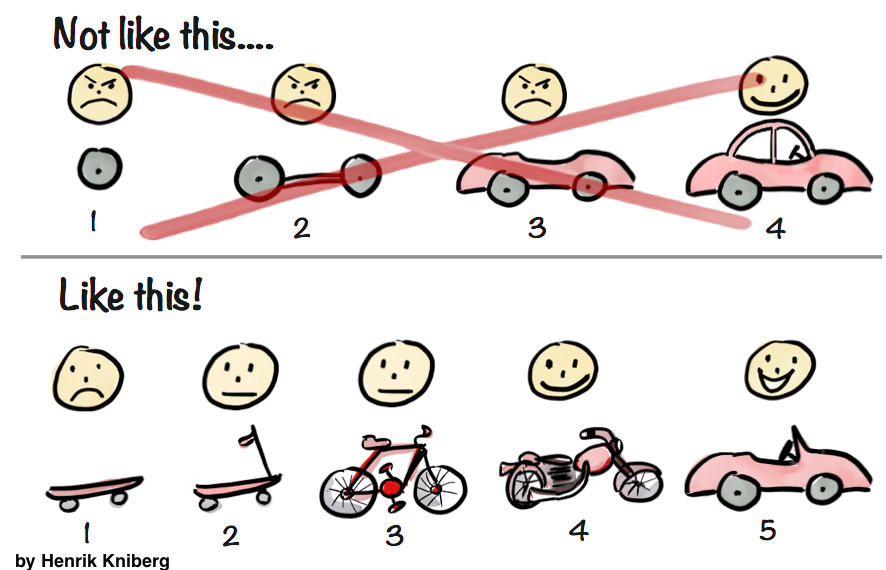
\includegraphics[width=1.00\textwidth]{images/mvp2.png}
   \caption[MVP]{MVP\\Each picture represents a stage in the development process (from left to right), with the client's face above, describing their mood\\Courtesy of \href{https://twitter.com/henrikkniberg/status/685474589539983360}{Henrik Kniberg}}
\end{figure}

Then, each developer would get assigned or choose a few features from the first Milestone until completion. Every morning, we would gather for a 10-minute stand-up meeting, during which everyone would say what they did the previous day and what is left to do, especially regarding the current day. Standing forces us to speak concisely and avoid wasting each other's time, since it is not as comfortable as being sat down.

\medskip

At the end of the Milestone's week, we would merge all the Pull requests resulting from the features, then review all together all the work done, conduct tests and create issues on GitHub to be resolved before starting the next Milestone. Eventually, we would readjust the remaining Milestones when needed.

\medskip

This would go on until completion of the final Milestone, which is supposed to bring all the features originally requested by the client.

\begin{figure}[H]
   \centering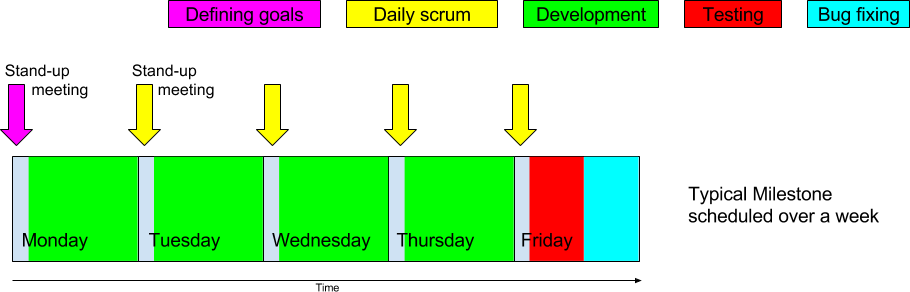
\includegraphics[width=1.00\textwidth]{images/scrum.png}
   \caption[Scrum]{A typical week at The Smiths}
\end{figure}

Sometimes, the part "Bug fixing" would require extra-time. In such a case, we would extend that part onto the next week, only assigning one person, so that the rest of the team could stick strictly to the rule "a Milestone per week". But that rarely happened fortunately.

\subsection{Mix them all}

As a brief conclusion, when thinking back at all the parts of our workflow, one can see that it is an entire whole in which GitHub plays a key-role. Being organized, knowing everyone's role and keeping in mind goals to reach are important as well, just like the tools we decided to go with. Furthermore, being able to release intermediate versions, quickly, allowed us to give constant feedback to the client, which is reassuring.

\medskip

This workflow is surely perfectible, but until now it has proved really efficient. Nevertheless, adapting Titanium apps, not to mention Titanium widgets, to automated tests is still a rather hard thing to do, even though there is an interesting tool developed for UI testing, called Calabash\footnote{\href{https://github.com/appersonlabs/TiCalabash}{https://github.com/appersonlabs/TiCalabash}}.
\chapter[Designing an API]{Designing a robust REST API}\label{chap:api}

Most of the time, the only purpose of an API is to give clients (a mobile application, a software program, a web browser, etc) access to a remote database (thus a server), in order for them to store data (or make complex calculations sometimes). The scheme is very simple: the server waits for incoming requests and responds accordingly. On the other hand, clients occasionally send requests, either to perform an action (saving, updating or deleting data), or to retrieve data.

\medskip

When it comes to designing and implementing (REST) APIs, I had always been seeking a standard to follow\footnote{Some people are trying to create a standard, see \href{http://jsonapi.org/}{http://jsonapi.org/}} or some best practices to apply. After doing loads of research, my colleagues and I finally came up with a scheme working pretty well.

\medskip

This part of the report assumes the reader has some knowledge of the HTTP protocol. It goes without saying that one must use HTTPS when dealing with APIs to ensure privacy. This way, everything will be encrypted and anyone sniffing the network will not be able to see the content of requests or responses.

\medskip

Before explaining what it is, let me first describe the process we went though, from understanding what is underlying (the very basic concept of HTTP) to the final API we wanted to build.

\section{REST}

In "REST API", "REST" stands for "\textit{Representational State Transfer}", which is the software architectural style of the web. Basically, this means that any REST API relies on the HTTP protocol (and by extension HTTPS). As a consequence, the first step I went through was to understand all the strengths and weaknesses of HTTP in order to use everything it has to offer. I will only be referring to HTTP version 1.1 in the coming lines, since version 2 is still hardly used overall, and quite badly supported.

\section{It is all about resources}

URLs\footnote{Uniform Resource Locator} represent resources. When designing an API, I had been thinking about it as resource containers. Every end-point should represent either a resource or a list of resources. Following this, \textbf{there must be two-end points per resource, the resource collection, and an individual resource within the collection}:

\begin{lstlisting}
/users
/users/{id}
\end{lstlisting}

The important thing here, is to understand that \lstinline|{id}| is a resource's unique identifier. For users, we retrieved these unique identifiers thanks to the \lstinline{/users} end-point (which had given us the list of users). So, \lstinline|/users/{id}| will give us all the details about \textbf{one resource}, the targeted user. The same rule applies for any other collection of resources.

\medskip

Moreover, resources can be imbricated, creating some kind of hierarchy, with an idea of "resources contained in a bigger set of resources", like in the following example, where messages belong to specific users:

\begin{lstlisting}
/users/{userId}/messages
/users/{userId}/messages/{messageId}
\end{lstlisting}

\section{Methods (also called verbs)}

One of the biggest strengths of HTTP is its verbs. The most popular are \lstinline{GET} and \lstinline{POST}. The latter is mostly used for asynchronous calls (AJAX) or forms in web pages, whereas the former is used every time a page is accessed or reloaded from a browser.

\medskip

For APIs, we mostly use PUT, GET, POST and DELETE. For example, this is how to create, get, update and delete a specific user:

\fakeshell
\begin{lstlisting}
POST   /users      # Create
PUT    /users/{id} # Create
GET    /users/{id} # Get
PUT    /users/{id} # Update
DELETE /users/{id} # Delete
\end{lstlisting}

Here, the important thing is that \lstinline{PUT} is used to create a specific resource (a user), whose identifier has been chosen by the client. Then, the second \lstinline{PUT} updates the newly created resource. When one wants to create a resource without specifying its identifier, one must use \lstinline{POST}. \textbf{\lstinline{POST} is only dedicated to creating resources}, unlike \lstinline{PUT} that will mostly be used to update, but can also be used to create.

\section{Understanding HTTP}

At this point, I need to add some explanation about the HTTP protocol. Every HTTP transaction (request or response) is made of three main parts:

\begin{itemize}
  \item An initial line
  \item Some headers
  \item The body, separated from the headers by a blank line
\end{itemize}

For requests, the initial line is made of a verb, a URL and the HTTP version used. On the other hand, for responses, it is a bit different: the HTTP version, a response status code and an English reason phrase describing the status code. For instance:

\code{An HTTP request}
\begin{lstlisting}
POST /users/123 HTTP/1.1
Host: my-api.com
Content-Type: application/x-www-form-urlencoded

name=Jon&lastName=Snow
\end{lstlisting}
\code{An HTTP response}
\begin{lstlisting}
HTTP/1.1 200 OK
Expires: Thu, 24 Sep 2015 19:36:25 GMT

Hello world
\end{lstlisting}
That said, let's get back to APIs.

\section{Transmitting data}

How can a client update a user on the server? What if someone wants to update their biography for example? Or wants to mention their age? Likewise, how does the server respond and send data back to clients? Here come the status codes and the body.

\medskip

Basically, clients need to send one type of information in the body: data to be put into the remote database (or processed), via a \lstinline{PUT} or \lstinline{POST} request. It can be either to create a new resource or to update it (it depends on the HTTP verb used).

\medskip

On the other hand, the server can send different types of information:

\begin{itemize}
  \item Via the status code:
  \begin{itemize}
    \item How the request was handled
  \end{itemize}
  \item In headers:
  \begin{itemize}
    \item Metadata
  \end{itemize}
  \item In the body:
  \begin{itemize}
  \item A resource or a list of resources, in response to a GET request.
  \item Some details about a resource newly created, in response to a PUT or POST request. For example, the resource's unique identifier or URL, to access this resource.
  \end{itemize}
\end{itemize}

As you can see, the body is only dedicated to the requested resources(s). That is all. All other useful information must be transmitted via the HTTP status code or headers.

\subsection{The status code}

Here are the most used status codes for an APIs, thus those we decided to go with:

\begin{table}[H]
  \begin{center}
    \noindent\begin{tabular}{ | r  l | l | }
      \hline
      Status code & Associated message & Used in response to\\
      \hline
      200 & OK                    & GET\\
      201 & Created               & PUT (when creating a resource), POST\\
      202 & Accepted              & PUT, POST\\
      204 & No Content            & PUT, DELETE\\
      301 & Moved Permanently     & GET, PUT, POST\\
      400 & Bad request           & Any\\
      401 & Unauthorized          & Any\\
      403 & Forbidden             & Any\\
      404 & Not Found             & GET, PUT (when updating), DELETE\\
      500 & Internal Server Error & Any\\
      \hline
    \end{tabular}
  \end{center}
  \caption[Main HTTP status codes used with APIs]{Main HTTP status codes used with APIs}
\end{table}

The HTTP protocol is very flexible, allowing us to use any non existing code if needed and relevant, when none of them fits our needs. That is why for the project \textsc{KopenVerkopen} (see chapter \ref{kvk}), we decided to add a few custom codes, within the range 550--599 (which are unused codes, according to the RFC\footnote{\textit{Request for Comments}, a document usually describing a protocol related to the Internet. For HTTP/1.1, see \href{https://tools.ietf.org/html/rfc2616}{tools.ietf.org/html/rfc2616}, even though it is been marked as obsolete (errata had been published since then).}).

\subsection{The body}

Sending parameters, from HTML forms, is pretty easy, it is a key-value thing, where parameters are separated by "\&", like this:

\code{The body of an HTTP request}
\begin{lstlisting}
firstName=Jon&lastName=Snow
\end{lstlisting}

However, out of the context of HTML forms, how to format the body? Well, one could say we could use the same key-value format, but actually, it is not a good idea. Let's see what options we have.

\subsubsection{A historic battle: XML vs. JSON or SOAP vs. REST}

We had two main options: XML or JSON. Nowadays, a lot of people use JSON. I will not try to defend JSON here, there are loads of debates on the Internet\footnote{\href{http://www.json.org/xml.html}{www.json.org/xml.html}}. To briefly sum it up, JSON brings efficiency, lightness and high-readability in a single format. Additionally, it is extremely easy to parse with any language, thanks to a great integration and a lot of support. It is definitely the most popular format when dealing with APIs. We can easily create a single object or an array of objects. \textbf{Basically, this is how we decided to go with JSON for all the APIs we would have to design.}

\subsection{A particular header}

Earlier on, I explained that the second part of every HTTP request is the headers section. Let me introduce one of them, probably the most important one: \textbf{\lstinline{Content-Type}}.

\medskip

Its only purpose is to specify what kind of data we are sending. Consequently, in our case, this header should be like:

\code{Real world example of an HTTP request containing \lstinline{Content-Type} header}
\begin{lstlisting}
POST /users HTTP/1.1
Host: my-api.com
Content-Type: application/json

{
    "name": "Jon Snow",
    "bad_guys_killed": 200,
    "skills":
        [
            {"name": "Warrior"},
            {"name": "Member of the Night's Watch"}
        ],
    "is_a_badass": true
}
\end{lstlisting}

Basically, its value is just a MIME type. To such a request, the response the server would send back:

\code{Example of a response sent by the server}
\begin{lstlisting}
HTTP/1.1 201 Created
Content-Type: application/json

{
    "id": 123
}
\end{lstlisting}

We can see that the server created the resource (thanks to the status code). It also gives us its ID, JSON-formatted.

\bigskip

\begin{center}
\noindent\rule{10cm}{0.4pt}
\end{center}

\bigskip

At this point, the API is able to do the four basic operations we needed (Create Read Update Delete), on any kind of entity, easily, thanks to a pretty format, JSON. End-points are semantic and hierarchically ordered. Everything is perfect. But...

\medskip

We are not taking advantage of all the strengths of HTTP (headers for example). And what if we want to apply some filters to our GET requests? Sorting? What about pagination? Those are all the sorts of questions we had been wondering about. More importantly, what about security? Authentication?

\section{Headers are metadata}

A great thing to consider is that the body must only contain the requested resource(s). Any other piece of information must go to the headers. Furthermore, we can create any header we want.

\subsection{Authentication}

There are two major concepts under the name of authentication.

\begin{itemize}
  \item Sign up/Log in/Log out: \textbf{user management}
  \item Authorization: \textbf{restricting the access to the API}
\end{itemize}

User management can be be achieved with cookies. This way, we can restrict some end-points to logged in users only.

\medskip

In parallel, we wanted to restrict our APIs to specific clients. One could say "Use basic authentication", but that did not really fit our need since it is not the original purpose of basic auth.

\medskip

Instead, what we came up with, is quite easy: creating as many HTTP headers as we wanted and sending (secret) keys on every request. For example, let's create a key to make sure we are accessing the right app, and another one to define the access level granted:

\code{An HTTP request containing custom security headers}
\begin{lstlisting}
POST /users HTTP/1.1
Host: my-api.com
Content-Type: application/json
Security-APP-ID: 123456
Security-Access-Level: 3

{
    "name": "Jon Snow"
}
\end{lstlisting}

Obviously, as I said in the beginning of this chapter, all of this would not make sense at all if we were not using HTTPS. We really do not want to expose such keys to anyone on the network.

\subsection{Location}

Another useful header is \lstinline{Location}. A good practice is to use it after creating a resource with \lstinline{POST}, to give back the location of the resource newly created. This way, no body is needed and our API can respond with a status code \lstinline{201 Created}, without a body. For example, after creating the user Jon Snow, we would get:

\code{An HTTP response giving back the location of the new resource}
\begin{lstlisting}
HTTP/1.1 201 Created
Location: https://my-api.com/users/123
\end{lstlisting}
The protocol and domain are optional, we could just send \lstinline{/users/123}.

\subsection{Other useful piece of information}

Basically, we can create as many custom headers as we want. A good practice with end-points returning a list of resources, is to give the total number of records in the database when relevant, via a header. We were doubtful about the relevance of such a practice, since we can programmatically count the number of results. But, as I will explain it in the next section, we are never going to return the full list of results in a single response.

\section{Pagination}

When returning a list of resources, above a certain number or results, it is a best practice to split responses in pages. It helps to reduce the waiting time and the weight of responses. Moreover, end-users might not need the whole list at once. Depending on the amount of details provided for each resource, a general rule would be returning between 100 and 1000 results per request as a maximum.

\medskip

Requesting a page is as simple as providing a query parameter:

\code{Requesting a specific page}
\begin{lstlisting}
GET /users?page=3
\end{lstlisting}

On the server side, we would just skip the \textit{<number-of-results-per-page>*<number-of-page>} first users. Pages start at 0.

\medskip

For instance, if we return 100 users per request, with page 0 we would skip no one and simply returns the first 100 users (from 0 to 99). On page 1, we would skip the first 100 users from our database and return the users from 100 to 199, and so on. But there is a problem...

\bigskip

Let's say we have 10 users in our database. Every \lstinline{GET /users} returns 3 users at most, \textbf{sorted by age}. In SQL, this would be something like:

\sql
\begin{lstlisting}
SELECT id, name, age FROM users ORDER BY AGE LIMIT 3 OFFSET x;
/* where x equals 3*<number of page> */
\end{lstlisting}
\code{} % reset language used
We would then have 3 pages and for each person, their id, name and age:

\begin{table}[!h]
  \begin{center}
    \begin{tabular}{ | l  | l | l | }
      \hline
      Page 0 & Page 1 & Page 2\\
      \hline
      45, Jon, 20   & 55, Alice, 30 & 99, Pete, 37\\
      87, Laura, 23 & 9, Bob, 33    & 1, Cindy, 39\\
      3, Jean, 25   & 2, Helen, 36  & 78, Max, 40\\
      \hline
    \end{tabular}
  \end{center}
  \caption[Example of 3 pages of result after API calls]{The 3 pages of results}
\end{table}

\noindent Here is a scenario:

\begin{enumerate}
  \item \lstinline{GET /users?page=0}: fine, we get results from Jon (id 45) to Jean (id 3).
  \item A new user (Mary) signs up on our website/mobile application, aged of 24.
  \item \lstinline{GET /users?page=1}: we get results from Jean to Bob. We got the same person twice (Jean), this is a problem.
\end{enumerate}

\noindent \textbf{What happened?}

\bigskip

As Mary is 24 and the API returns results sorted by age, Mary would be returned on page 0, which shifts Jean to page 1.

\medskip

A good way to solve this problem is to create a pagination based on an entity (here, a user). Instead of requesting a particular page, we would say to the API "give me results after this user" or "before this user". Let me explain it by replaying the scenario:

\begin{enumerate}
  \item \lstinline{GET /users}: no pagination specified, fine, we get results from Jon (id 45) to Jean (id 3)
  \item A new user (Mary) signs up on our website/mobile application, aged of 24.
  \item \lstinline{GET /users?pageAfter=3}: since the last person of our previous results had an id of 3, we request the users after that id. This way, we make sure we will not get duplicated results.
\end{enumerate}

For the project \textsc{KopenVerkopen} (see  chapter \ref{kvk}), while designing the global architecture of the project, we faced that problem. This is how we solved it.

\medskip

Two last pieces of advice we also had to consider:

\begin{itemize}
  \item Always enable pagination, even if the entire collection is small and will never grow. Like this, APIs' users will not get lost. The API remains consistent.
  \item If a page returns this entire collection, one should always use the status code 200. Otherwise, 206 ("\textit{Partial Content}")
\end{itemize}

\section{Filtering and sorting}

Every end-point that returns a list of resource should allow filtering on fields, as well as sorting. The following request should be possible:

\code{Filtering and sorting on an HTTP request}
\begin{lstlisting}
GET /users?country=US&age=21&sortBy=name
\end{lstlisting}
We request all the users from the US, aged of 21, sorted by name. The inner mechanism is up to the developers.

\section{Conclusion}

Building an efficient API involves many aspects to consider, and most of all, requires a good knowledge of HTTP. It is time-consuming at first sight, but once you know what you are doing, what your needs are in terms of features, it is pretty straightforward. Considering all aspects right at the beginning, like security or the database architecture and how you would like to expose it, is key. That is what is called designing an architecture, and one should pay heed to it. When properly and carefully done, the API implementation job is fairly easy.

\medskip

This whole process of gathering information was worthy. We had to go through many talks (videos), tutorials or RFCs to eventually get a good understanding of what a "REST API" really meant.
\chapter{Bearleaders}

Bearleaders is the name of a project I was assigned as soon as I arrived in the company. It was a project born thanks to a friendship between Wienke and a good friend of him, who basically became our client. This project was supposed to be my main mission within the Smiths, with a duration of at least two months, up to four.

\medskip

For several years, she (the client) had been running a small business: \textbf{a website gathering all the points of interest in the main cities of Europe}. The spots were sorted by categories (food, sleep, bars, ...). Anyone was able to sign up on this website and add spots, letting other users see them. Consequently, logged in users were able to browse across all the spots uploaded by users, get details, comment, etc. It was a kind of guide for Europe, on the Internet. Its main advantage was that it was free with a fairly important community.

\medskip

But some day, she came to Wienke with an idea in mind, knowing what \textsc{The Smiths} was. She wanted to "upgrade" her website and push her business to the next level. \textbf{Actually, she wanted a mobile app to replace her aging website, available on iOS and Android.}

\medskip

Both Wienke and her agreed on a time frame of two months, for a really fair price. The road map was pretty simple:

\begin{enumerate}
  \item Understanding the need
  \item Designing the mobile app while writing specifications
  \item Coding
  \item Tests, improvements and publishing
\end{enumerate}

This was an entire project from scratch. \textbf{We had to create the back-end\footnote{Everything related to the distant server, which generally stores data and provides services to clients (such as a mobile app or a website). It is usually made of a database and an API.}, take care of the old database and create a new one, develop the API and a back-office as well. In parallel, we were obviously also responsible for the development of the mobile app on Android and iOS.}

\section{Understanding the need}

When I arrived, in early September 2015, Wienke told me I would be in charge of the entire project, working jointly and closely with our designer, Wessel \textsc{Versluis}. However, after a couple of days, I had met the client only once, whereas Wienke and Wessel had many times. I found that quite weird as I was supposed to be responsible for the project. The only reason I had been given was that me attending the meetings was not necessary at that stage. Later, I understood that they were actually trying to figure out what the client really expected from us.

\medskip

Finally, after a few weeks, I had a better understanding of the project, the idea behind it, the final goal, and so forth. Thanks to the tight collaboration between Wessel and me, things were starting to move progressively. As I said above, the client wanted a fresh new version of her website made available as a mobile app.

\medskip

After being granted access to the old codebase of her website, it turned out to be rather obsolete and unmaintainable, regarding the frameworks used and the general quality. The database was a mess as well, really hard to maintain. I could foresee a huge amount of work coming ahead of me. In addition, she wanted most of the existing features to be somehow exported to the app, as well as adding brand new features.

\section{Designing the app}

In late September, meetings were still scheduled on a regular basis, but only involving Wessel and the client. These were mainly about design concerns. As for me, things were quite clear, from a technical point a view solely. However, after every meeting, I was getting news from Wessel about new features to add or remove. As far as I am concerned, I found it really inappropriate. In my opinion, the client was just overthinking and could not help herself from that. She was merely unable to agree on an ultimate product because of a poorly prepared plan.

\medskip

Wessel did a really good job figuring out which features were fundamental and which ones were not. He also proved a great ability to sketch mockups quickly, providing me with PNG exports as soon as the client would agree on them.

\medskip

On my side, I was designing the whole architecture of the project with everyone else's help, to finally start writing down the specifications.

\section{Specifications}

At some point, I had enough clues to start writing the specifications, although we still had not agreed on anything completely definitive. The contract was non-existent, which I though was not a good sign whatsoever.

\medskip

It had been decided to host the back-end source code on \href{https://www.parse.com}{parse.com}, and build the API on top of that. In addition, we would obviously use Titanium as a mobile app development platform for the mobile app, enabling us to use the same codebase for both Android and iOS.

\medskip

\href{https://www.parse.com}{Parse.com} offers, for free (with certain conditions, but it fitted our needs perfectly), a whole hosting solution and a set of tools to deploy server code flawlessly, thanks to a CLI. Moreover, they also provide their database made in-house, which in fact is a sort of more abstracted layer, on top of a regular database underneath (MongoDB\footnote{A database management system (DBMS) slightly different from conventional systems (relational systems)}). Parse is marketed as a BaaS\footnote{\textit{Back-end As A Service}} but it can be considered as a PaaS\footnote{\textit{Platform As A Service}} since the tech stack is very similar to other service providers like \href{https://www.heroku.com/}{Heroku}. Just like on any regular hosting provider, one can deploy source code simply by typing a command in a terminal. In the code, communication with Parse's database is established thanks to an API (a few JavaScript functions) provided by Parse, called "Cloud Code"\footnote{\href{https://parse.com/docs/cloudcode/guide}{https://parse.com/docs/cloudcode/guide}}.

\medskip

Regarding the API, as our whole stack relies on JavaScript, we naturally decided to go with \href{http://expressjs.com/}{Express.js} which is one of the greatest minimalist frameworks, used to build APIs insanely fast, in solely a couple of lines. Besides, it is even natively embedded in Parse, which means that Parse can run an Express.js server.

\begin{figure}[!h]
   \centering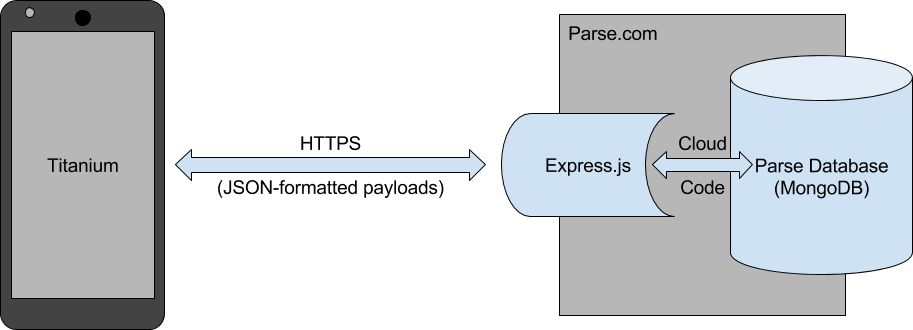
\includegraphics[width=1.00\textwidth]{images/bearleaders.png}
   \caption[Bearleaders' architecture]{Bearleaders' architecture}
\end{figure}

\section{API}

While writing specifications, I identified different type of entities (for example \textit{users}, \textit{spots}, \textit{categories}). As I wanted the API to be serviceable and convenient, I decided to reflect the entities through the API. That was the time I made loads of research about APIs and eventually ended up writing a blog post\footcite[See the reference][in the bibliography]{api_my_blog} about that topic, which has massively contributed to the writing of chapter \ref{chap:api}, in this report.

\medskip

I will not explain any further how I built the API as everything has already been told in the chapter \ref{chap:api}. As a matter of fact, the only purpose of that API was solely to reflect and expose the underlying database, allowing logged-in users and administrators to perform additions or edits, depending on their rights.

\section{Exporting the old database to the new back-end}

Upon completion of the specifications, I was focused on the development of the API. I was going back and forth as I would notice problems or potential issue in my design. Then came the tricky part.

\medskip

This part was not easy at all and yet, really interesting. From a MySQL\footnote{A popular database management system (DBMS)} dump sent to me by our client, I had to export valuable data to our new hosting provider, \href{https://www.parse.com}{parse.com}. However, as part of the initial requirements, only a small portion of data was truly valuable to our client. We discussed that over emails or during meetings, over and over. Basically, she wanted to keep genuine users, those loyal to her website since years, those who were deeply involved into the community of spot finders. On the other hand, she also wanted to keep only the spots added by herself and those users. Nevertheless, she asked us to edit the spots a bit, mostly rearranging categories, making sure the GPS location was accurate, a description was existent, and so forth.

\medskip

In order to achieve this, I simply imported the dump into a local MySQL database on my computer. Then, I wrote quite complex SQL\footnote{\textit{Structured Query Language}, the mainly used language to request most DBMSes. Some queries are in the appendix \ref{bearleaders-sql}} queries -- complex because I had to handle to inconsistency of the old database -- inside a NodeJS script to finally send valuable data to Parse.com, using the API I had just created. It took me around ten days to achieve this.

\section{The back-office}

A back-office is more or less an interface (as a website, most of the time) to administrate a product, a website. For example, an administrator can use a back-office to manage users, upload blog posts, etc. It is basically a restricted area only available to privileged users (admins).

\medskip

Here, the back-office was supposed to offer the same capabilities as the previous one (the one used to manage her old website). But obviously, adapted to the new product, taking into consideration the changes we would bring.

\medskip

Consequently, I decided to develop a MVP with few features but still, usable. I wrote plain old JavaScript, and used in the meantime a library\footnote{\href{http://www.editablegrid.net/}{http://www.editablegrid.net/}} found on the Internet, to manipulate tables and grids of data and easily make them editable. The back-office was restricted to an administrator using special credentials. Then, once logged in, the JavaScript code would use the API I had developed to display and edit data.

\section{Cancellation}

Late October 2015 already and meetings are still ongoing with Wessel, usually every two weeks. At this stage, he was still trying to figure out how to please our client. Iterating over and over about which features are relevant for the MVP, determining which ones are useless, trying to make everything fit in a two-month schedule at a fair price. But unfortunately, the two months had already been reached and we still had not agreed on anything. Worse, no contract had been signed, as it was a friendly agreement. The outcome was very predictable.

\medskip

We were all getting tired because of non-sense decisions. One week she would settle for a set of features. The following week, she would reconsider everything. The money and time constraints made it all even more difficult to handle. I was completely unused to such methods. It was really getting on everyone's nerves.

\medskip

One day, Wienke came to us, after reflecting quite much, decided to end it all. He gave her a ring and within a few minutes the two previous months vanished. She told him it was completely unexpected to her, pretending to realize that things were going wrong, out of the blue.

\medskip

Even a long forecasted cancellation is not easy to accept, but there is always something to learn from it, by analyzing it, looking back and more importantly, putting it into perspective.

\section{Where we failed and why}

Although we all knew the reasons of such a failure, we still analyzed the situation and the ins and outs, in order to get a deep insight and avoid alike scenarios in the future. The past two months were thoroughly reviewed. That is a crucial part for an agency, understanding why such events occur, in order to be more preemptive in the future and prevent such things from happening.

\subsection{Design before features}

From my point of view, we tried to carry out the whole project badly, the wrong way. After few meetings with everyone involved, despite the features were still completely unclear to us, our designer started working closely to the client, meeting her almost every week.

\medskip

At first sight, we thought we got it, the project appeared pretty obvious and simple to us, only a handful of features, nothing too big. Just a regular project, one of those The Smiths were used to. I guess it is also one of the reasons why Wienke agreed on that friendly agreement. However, as I said, soon enough (in mid-September perhaps), we felt something was wrong. Meetings were lingering way too much about details, the client were reconsidering again and again. It was really baffling.

\medskip

The right way to proceed, in my opinion, would have been to ask the client for specifications, discuss about them during a meeting or two, and finally sign a contract with goals and features clearly written down. This way, the client would be forced to carry out the whole without saying a word, instead of iterating repeatedly. Then, I would not have been stuck waiting for a final agreement, as it was. Wessel and I would have been able to work independently, in parallel. At some point, in October, as I was done with the API and back-office, all I could do was waiting for the definitive features, the design and thus the assets, to really start coding the mobile app.

\subsection{Overiterating \& Overthinking}

Giving the client too much power lead us to a failure, inevitably. Of course we are an agency and we are supposed to comply with our clients' requests, but that went definitely too far. To stick to the original time frame allocated to her project, every week she would come up with new ideas, features to remove and some other ones to add. Tinkering, that is what she was actually doing without being aware of it.

\medskip

To sum up, the lessons learnt from that project are pretty simple:

\begin{itemize}
  \item Do not do business with friends, unless there is a real contract signed by both parties. If you do so, carry it out treating the client as it, not as a friend.
  \item Ask for specifications from the client; as an agency our job is not to guess the need (except if we want to provide consulting services as well, which is not the case with The Smiths).
  \item Agree on something quickly, cause time flies! And time is money (especially for an agency). The signed agreement should describe clearly enough the goals and features expected.
  \item Don't overpromise on the timeline, for example, try to cram a 6-month project into a 2-month timeframe
  \item Don't offer discounts even to friends: charge the right price
\end{itemize}

\section{Conclusion}

There is no real conclusion for this project as it was aborted. However, it was a good introduction to the tools used at The Smiths, like \href{http://www.parse.com/}{Parse.com}, \href{https://travis-ci.org/}{Travis-ci.org}, and above all, Titanium, in spite of the fact that I was mainly focused on the specifications writing -- which was a good practice as well.

\medskip

Nonetheless, the interesting part here was the project management, how it was handled throughout those two months. This internship was my first experience in an agency, what is more a startup agency. As one might guess, there is no magic recipe to succeed. The Smiths, though a young company, had already had some experience with clients management but this case was a new one. And we all learnt from it. Ultimately, it strengthened the team and sharpened our motivation. As of that moment, The Smiths would be cautious and would choose clients more neatly.
\chapter{KopenVerkopen}\label{kvk}

"KopenVerkopen", which literally means "BuySell" in English, is an internal project started in early Summer 2015. It is supposed to be a mobile alternative to \href{http://www.marktplaats.nl/}{marktplaats.nl}, which is the Dutch equivalent to the French website \href{http://www.leboncoin.fr/}{leboncoin.fr}.

\medskip

Pierre and Matthias were working on that project mainly during their "spare time", which basically was either when their client projects were not late on schedule or when the clients were \textbf{not} putting them under pressure because of bugs, issues or enhancements -- which happened rarely. Consequently, that project was still in an early stage and not much progress had been made. As soon as my project Bearleaders was canceled, I was reoriented to KopenVerkopen.

\section{Why an internal project}

The original idea behind that mobile application was the show to potential clients what the Smiths was able to do. As a development agency, we have a portfolio\footnote{\href{http://www.wearesmiths.com/}{www.wearesmiths.com}} listing all the projects we had been working on. Thus, they thought it would be a great thing to add a home-made app on it, just to show off.

\medskip

In the meantime, Pierre and Matthias saw that as the opportunity to try new technologies or libraries, so that we would improve our skills with no risk as the client was... us. Just like a playground, it was meant to carry out experiments of any type with Titanium as well as experiments in mobile development in general.

\section{What it is}

KopenVerkopen is, as I said, a selling app, for individuals. The concept is pretty simple: anyone can download the app and then easily log in using their Facebook account. Then, the user can either browse through items for sale or sell one of their items. The feed of items on sale can be filtered using different filters, like sorting from the closest buyer to the farthest one, according to the GPS location.

\medskip

When showing interest for an item on sale, the interested person is added to a stack of potential buyers. The owner of the product is then introduced to the first person of this list thanks to a conversation popping up on their screens, in a specific section of the app. The two people can now discuss about the sale itself. At any time, one of them can cancel the sale, which would remove the potential buyer from the list of interested people. In such a case, the owner would be introduced to the next potential buyer thereafter.

Finally, when both parties agreed on the sale, the owner can mark the item as "sold".

\medskip

Users can also manage their profile with a few basic options. The profile picture is the same one as on their Facebook profile. Furthermore, on the profile page, several shortcuts are available (see the figure \ref{tabs-kvk} right below).

\begin{figure}[H]
   \centering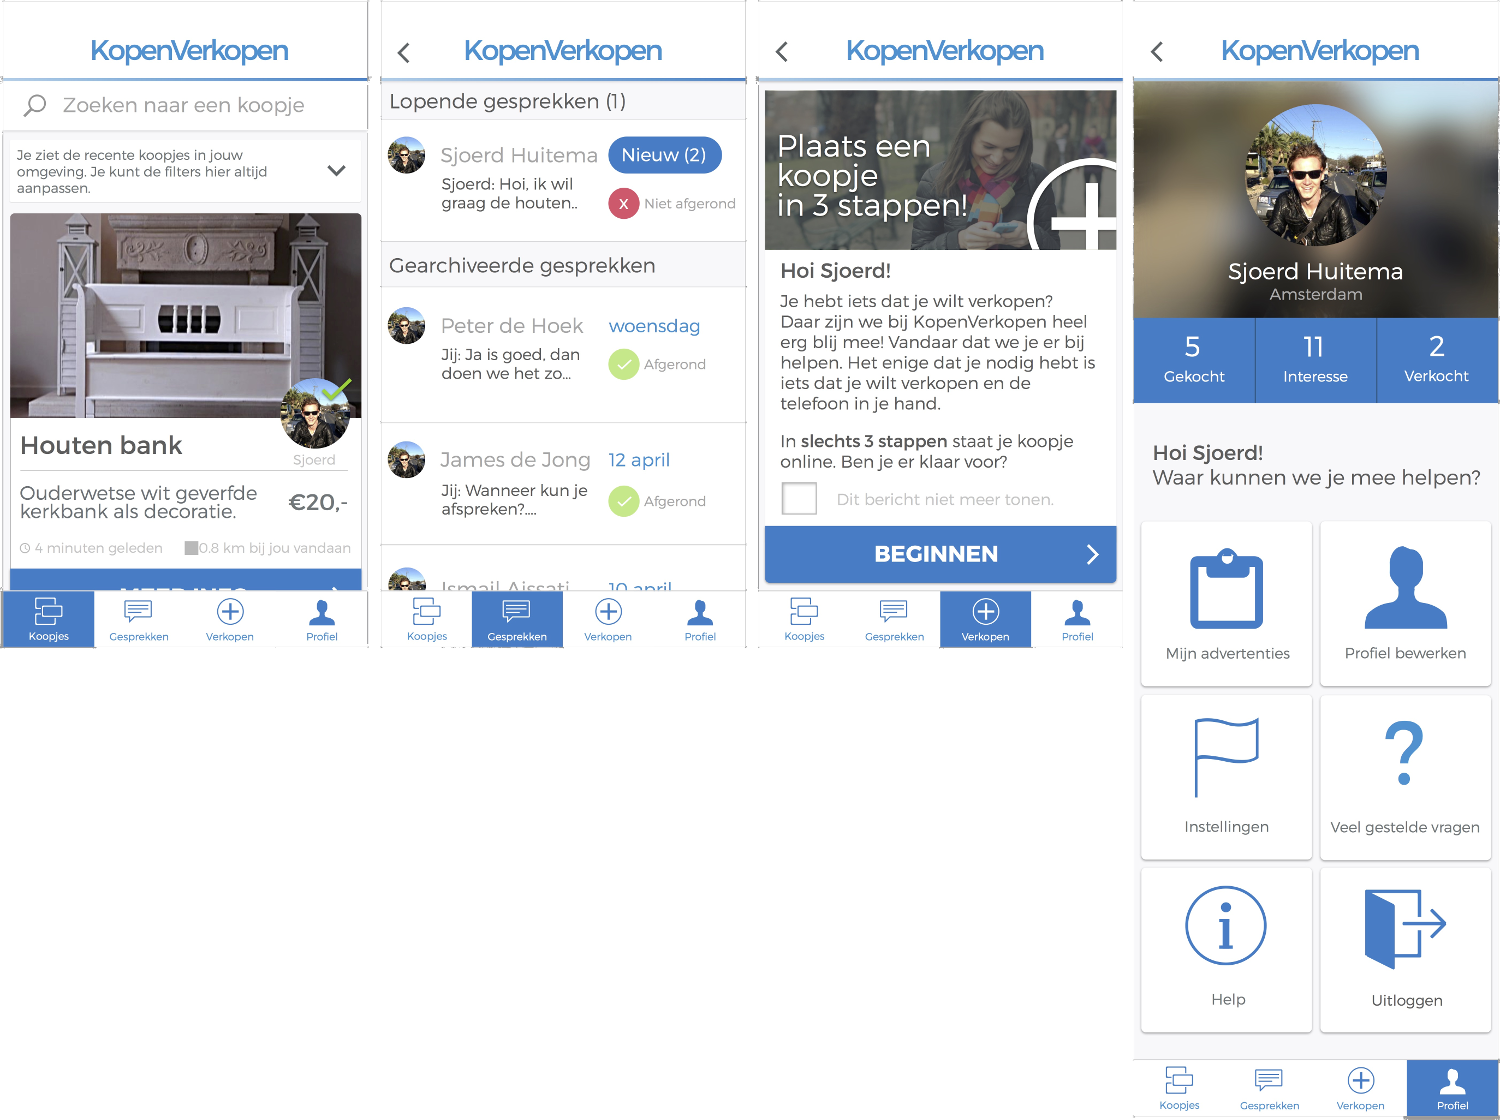
\includegraphics[width=1.00\textwidth]{images/kvk-tabs.png}
   \caption[The four main tabs of KopenVerkopen]{The four main tabs of KopenVerkopen\\From left to right: Feed of items on sale, Conversations with buyers/owner, Sell a new item, Profile and options}\label{tabs-kvk}
\end{figure}

\section{Road map, Strategy \& Reality}

The road map which seemed to be the most doable and realistic is as follows:

\begin{enumerate}
  \item Choosing carefully which features are relevant and needed (everyone)
  \item Designing the app (Matthias and the designer, Wessel)
  \item Writing the specifications formally (plus designing the UI\footnote{\textit{User Interface}})
  \item Coding (this part is a big one, hiding many sub-parts and iterations)
  \item Publishing
\end{enumerate}

\medskip

In parallel of the step 4, a lot of refactoring would be done on a regular basis, as well as code review sessions. Code reviews are meant to make sure everyone is heading in the right direction, and also to improve someone's code so that this person can learn from others. On the other hand, the goal of refactoring is to keep "innovating", improving our code, getting ride of obsolete code, and so forth.

\medskip

This schedule is somewhat simple and yet commonly encountered among software development. Nothing too much, as it would be an internal and experimental project. The allocated time was quite unsure, as we foresaw a lot of refactoring. Moreover, we would only work on that project during our "spare time", when client projects would wind down.

\medskip

When I arrived, back in September, the three first steps had almost already been conducted. The team was still polishing a bit the architecture, from time to time. Actually, the project had almost been paused. As of late October, it suddenly resumed, mostly because Bearleaders had been discontinued.

\medskip

During the first week "post-Bearleaders", I familiarized myself with the project, discovering its architecture, finding out what has been done so far, what was left to be done, and so forth. The specifications were available on our GitHub repository, mockups had also been created by Wessel. Soon enough, I noticed some issues in the current API and database\footnote{Parse.com does not provide a real database in the usual sense of the word. Instead, it is an abstraction of the underlying used MongoDB. But yet, developers -- us -- have to create sorts of simplified tables with typed columns. There are no triggers, no stored procedures, no constraints (not event \lstinline{PRIMARY KEY}, the system creates automatically a primary key for each row, with no possibility of deletion): all of them have to be written in specific files called "hooks", which are run before or after insertions automatically.}. I started to discuss it with Matthias and, as it often happens after a long period of inactivity, we were all agreed that there were few glitches that needed to be fixed. That was when we decided to go back to step 2. We did not need to edit the specifications as our changes would not have any effect on the mobile app itself.

\section{Involvement}

\subsection{API}

For approximately one or two weeks, I reused most of my blog post\footcite[See the reference][in the bibliography]{api_my_blog} about APIs to rethink ours. Matthias and I actually bought a set of whiteboard sheets to build a huge (4-meter long x 2 meters) whiteboard next to our desks, on a wall. We used it to write down our database structure as well as our API endpoints, linked to actions performable by users in the app. After this brainstorming period, he reflected all the changes to the back-end code and I did the same for the mobile app code.

\subsection{Example of a widget: ts.chat2}

In the meantime, I also updated a widget I had started in September, called "ts.chat2" which in turn is an upgraded version of "ts.chat".\\
"ts.chat" was a quite simple chat widget developed by Matthias which provided a minimalist -- though working like a charm -- UI for text messages, just like any SMS app. However, his widget used two modules to bring more features which turned out to be a problem: they were not very up-to-date and they introduced issues with newer versions of Titanium. I decided to get rid of those dependencies and develop a new widget, directly inspired from Matthias' one. It was also a great opportunity to explore widgets and their capabilities. As a reminder, widgets bring modularity which is a true strength of Titanium.

\begin{figure}[H]
   \centering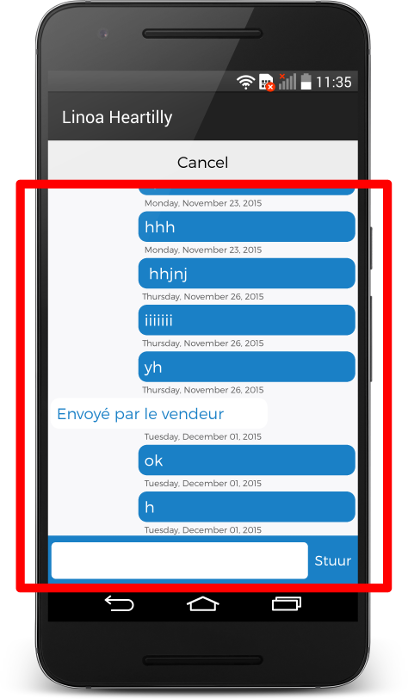
\includegraphics[width=0.45\textwidth]{images/tschat2framed.png}
   \caption[KopenVerkopen -- ts.chat2]{The red square shows the widget, included in a window}\label{tschat2pic}
\end{figure}

The widget receives a Backbone collection\footnote{\href{http://backbonejs.org/\#Collection}{http://backbonejs.org/\#Collection}} containing messages. It iterates through them in order to display them, from the oldest (on top of the screen) to the most recent. It also offers an input text field so that the user can add messages.

\medskip

The widget can trigger two distinct Backbone events:

\begin{enumerate}
  \item \lstinline{moremessages}: when the user scrolls to the very top of the screen
  \item \lstinline{newmessage} when the user has typed a message and sent it
\end{enumerate}

The first event is intended to fetch more messages from the server (older messages). The second one basically says that a new message is about to be sent (it also provides the message as a second argument, see the last line below):

\javascript
\begin{lstlisting}
var newmessageEvent = {
    message: $.typingArea.value,
    created_at: new Date(),
    success: function () {
        $.typingArea.value = "";
        _resizeTypingArea();
        $.sendBtn.touchEnabled = true;
        scrollToBottom();
    },
    error: function () {
        $.sendBtn.touchEnabled = true;
    }
};
$.trigger('newmessage', newmessageEvent);
\end{lstlisting}
Nevertheless, it is the responsibility of the developer to take care of that message.

\medskip

This widget works thanks to \textbf{data-binding}, a powerful concept, prominent within Titanium and deeply built-in\footnote{\href{http://docs.appcelerator.com/platform/latest/\#!/guide/Alloy_Data_Binding}{http://docs.appcelerator.com/platform/latest/\#!/guide/Alloy\_Data\_Binding}}. Basically, it is like linking a model or a collection of models (here \lstinline{Message}) to a view. As a result, the view would get automatically updated as soon as the model would change.

\medskip

In addition to the inner mechanism to handle messages, the widget offers some kind of customization. When included in a window, a few colors can be specified, for instance:

\begin{lstlisting}
$.chat.init({
    // Alloy.CFG.COLORS.x are defined in a global conf file
    messages: Alloy.Collections.messages, // The collection to use for Data Binding
    backgroundColor: Alloy.CFG.COLORS.WHITE_DARK,
    backgroundColorLeft: Alloy.CFG.COLORS.WHITE,
    colorLeft: Alloy.CFG.COLORS.BLUE,
    ...
    sendButton: { // Configuration for the button at the bottom right
        title: 'Stuur',
        borderRadius: 5,
        ...
    },
    typingArea: { // Configuration for the input text
        color: Alloy.CFG.COLORS.BLUE,
        ...
    },
    ...
});
\end{lstlisting}

\subsection{Entire app}

I got involved in other widgets (ts.prettymenu\footnote{\href{https://github.com/TheSmiths-Widgets/ts.prettymenu}{https://github.com/TheSmiths-Widgets/ts.prettymenu}}, ts.camera\footnote{\href{https://github.com/TheSmiths-Widgets/ts.camera}{https://github.com/TheSmiths-Widgets/ts.camera}}, and others not publicly available), but not as much as with \textit{ts.chat2}. Consequently, I will not detail them in this report.

\medskip

In summary, in chronological order, I have worked on:
\begin{itemize}
  \item \textbf{The conversations}: creating a new widget, updating the UI, inserting the widget, making sure it was working flawlessly.
  \item \textbf{Translations}: the app has been designed to support three languages (Dutch, English and French). I helped to translate some parts of the app.
  \item \textbf{Refactoring}: after the big decisions we had made regarding the back-end (API and data tables), new models had to be created based on the old ones. It also implied migrating the local databases (SQLite is used as a database for apps in both Android and iOS).
  \item \textbf{Polishing the UI}: conversations were reshaped many times to fit at best Wessel's design
  \item \textbf{Adding features to conversations}: I added a handful of features to the app, like two buttons to either cancel or sell an item
  \item \textbf{Bug fixing}: particularly in the dashboard (for some reason the menu was pretty bugged)
  \item \textbf{Adding features to the app}: logout, popups at different points (I had to create a widget for it by the way, see the figure \ref{popup} below), sharing capacities (on social media)
  \item \textbf{Bug fixing}: mainly on iOS, as I was developing on Android first
\end{itemize}
\begin{wrapfigure}{r}{0.4\textwidth}
  \vspace{-10pt} % hack
  \begin{center}
    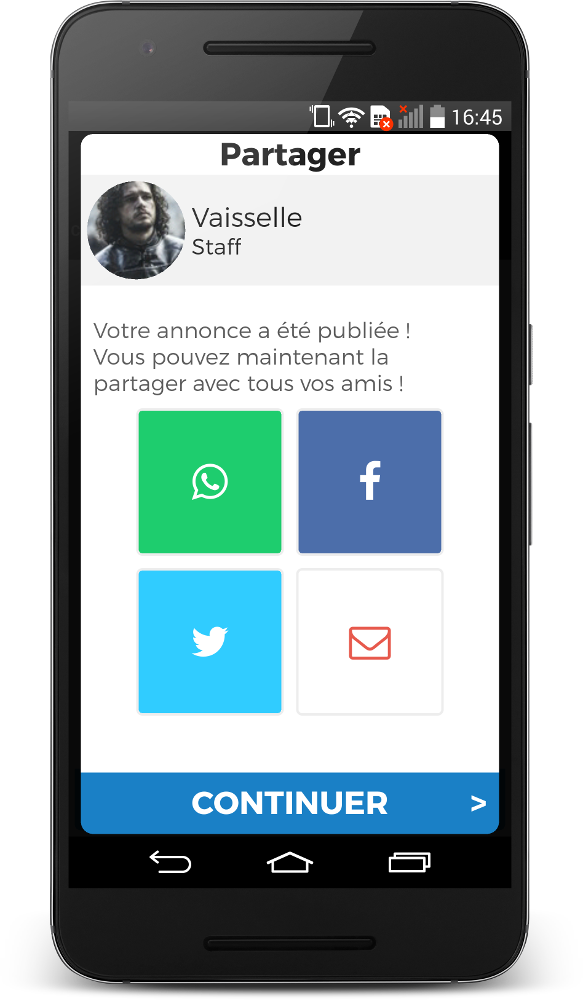
\includegraphics[width=0.35\textwidth]{images/popupframed.png}
  \end{center}
  \caption[KopenVerkopen -- Popup]{The popup showing social media icons}\label{popup}
  \vspace{-60pt} % hack
\end{wrapfigure}

In total, I had been spending roughly one week in September, and a whole month (from November, \nth{6} to December, \nth{9}).

\section{Current state and outcome}

As of early December, the project has been paused because of a new client project (see chapter \ref{tesco}). The back-end is fully operational and still running. The app is almost done. Most of the features have been implemented, a few ones excepted. However, there is still a lot of polishing to do and several glitches to fix. Although the app is in an advanced state, I would say that a bunch of months (perhaps two or three, tops) are yet to be spent working, on condition that two developers would work on it at least.

\section{Conclusion}

This project was really interesting as I had quite a lot of responsibilities, or a least the freedom to take decisions. Since it was an internal project, no money nor reputation was at stake. It was truly a deep-dive into Titanium. I really had the time to get a full overview of the entire framework (its advantages and drawbacks). In the meantime, it was a chance for me to contribute to the community by giving away widgets I had developed, or merely improving existing ones.

\medskip

After such an intense period dedicated to Titanium, I was able to weight the pros and cons regarding cross-platform mobile development, and more precisely Titanium. I had started to adopt techniques and best practices used by my colleagues to maintain a homogeneous code. More and more, I was feeling confident with JavaScript. That was somehow the pinnacle of my internship as I was gaining more experience everyday and learning from my colleagues efficiently. Our workflow had proven to be useful, it was bringing daily efficiency.
\chapter{DC Comics}\label{tesco}

This is the last project I have worked on. It was, by far, the most funny to do and the most challenging. It required Pierre and I working almost full-time on it, for more than a month (except during Christmas break), whereas Matthias was splitting his time between this project and \textit{The Things Network}\footnote{\textit{The Things Network} is a gigantic project initiated by Wienke during Summer 2015. It is a foundation aimed at building "\textit{a global open crowdsourced Internet of Things data network.}". In November 2015, they successfully raised €295.331 on the crowdfunding platform Kickstarter (\href{https://www.kickstarter.com/projects/419277966/the-things-network}{www.kickstarter.com/projects/419277966/the-things-network}). Since then, Wienke has been spending most of this time on this project. Matthias was invited to join the project as well, helping build the network itself. More information can be found on their website \href{http://thethingsnetwork.org/}{thethingsnetwork.org}.}.

\medskip

In early December 2015, Pierre found a new potential client thanks to someone working in our open-space at Rockstart. The deal, through very constraining, was worthwhile. \textbf{We had a twenty-day time frame of intense development for a few thousands euros.} At first glance we thought the deadline would be impossible to meet. However, full of motivation, Pierre and Wienke signed the contract with the company.

\section{Goal}

Our client is a big global company, which works in tight collaboration with DC Comics. They decided to launch a temporary event for the employees, a sort of contest. Employees can download a mobile app either on the Apple Store or Play Store. The app is restricted to some employees only, depending on their living country and on the store they work at. After providing credentials, the employees get logged in. Then, they can scroll through a feed of uploaded funny pictures, or create one as well. Creating a picture is the funniest part. First, you have to take a selfie of you. Then, your photo appears in an egg shape. You can add a background and amusing items all over your face, turning you into some sort of super hero. When you are done, you can upload your picture with a description and a custom super hero name.

\medskip

At the end of the contest, a group of designated people (from the company) acting as a jury will review each picture and pick out the best ones. The uploaders will likely be awarded.

\medskip

Uploaded pictures can also be reported as inappropriate by anyone, in order to prevent abuse. Once a picture has been reported at least five times, it will no longer show up in the feed and will be kicked out of the contest.

\section{Schedule}

For this project, we used \textsc{SCRUM} (agile method) very seriously. We had received highly detailed specifications so defining goals and a schedule was pretty straightforward. First, Matthias planned three Milestones over three weeks (one per week). He kept the last week of our four-week schedule free, just in case, as he somehow foresaw delays.

\medskip

The project started around mid-December and the delivery date was set for some day around the \nth{22} of January. Taking into consideration the winter break, we had more or less four weeks of development ahead of us.

\medskip

As I said in the section \ref{agile-methodology}, every morning we would do a ten-minute "stand-up meeting", talking about what had been done and setting new objectives for the current day. GitHub was the central point of everything. We used it as an agenda and a bug tracker. Our Git workflow proved here, once more, that it was well designed enough to allow us to improve our productivity. \textbf{In total, we submitted 46 Pull Requests and merged 247 commits into \lstinline{master}}. And all of this in one month.

\section{Development}

\begin{figure}[H]
   \centering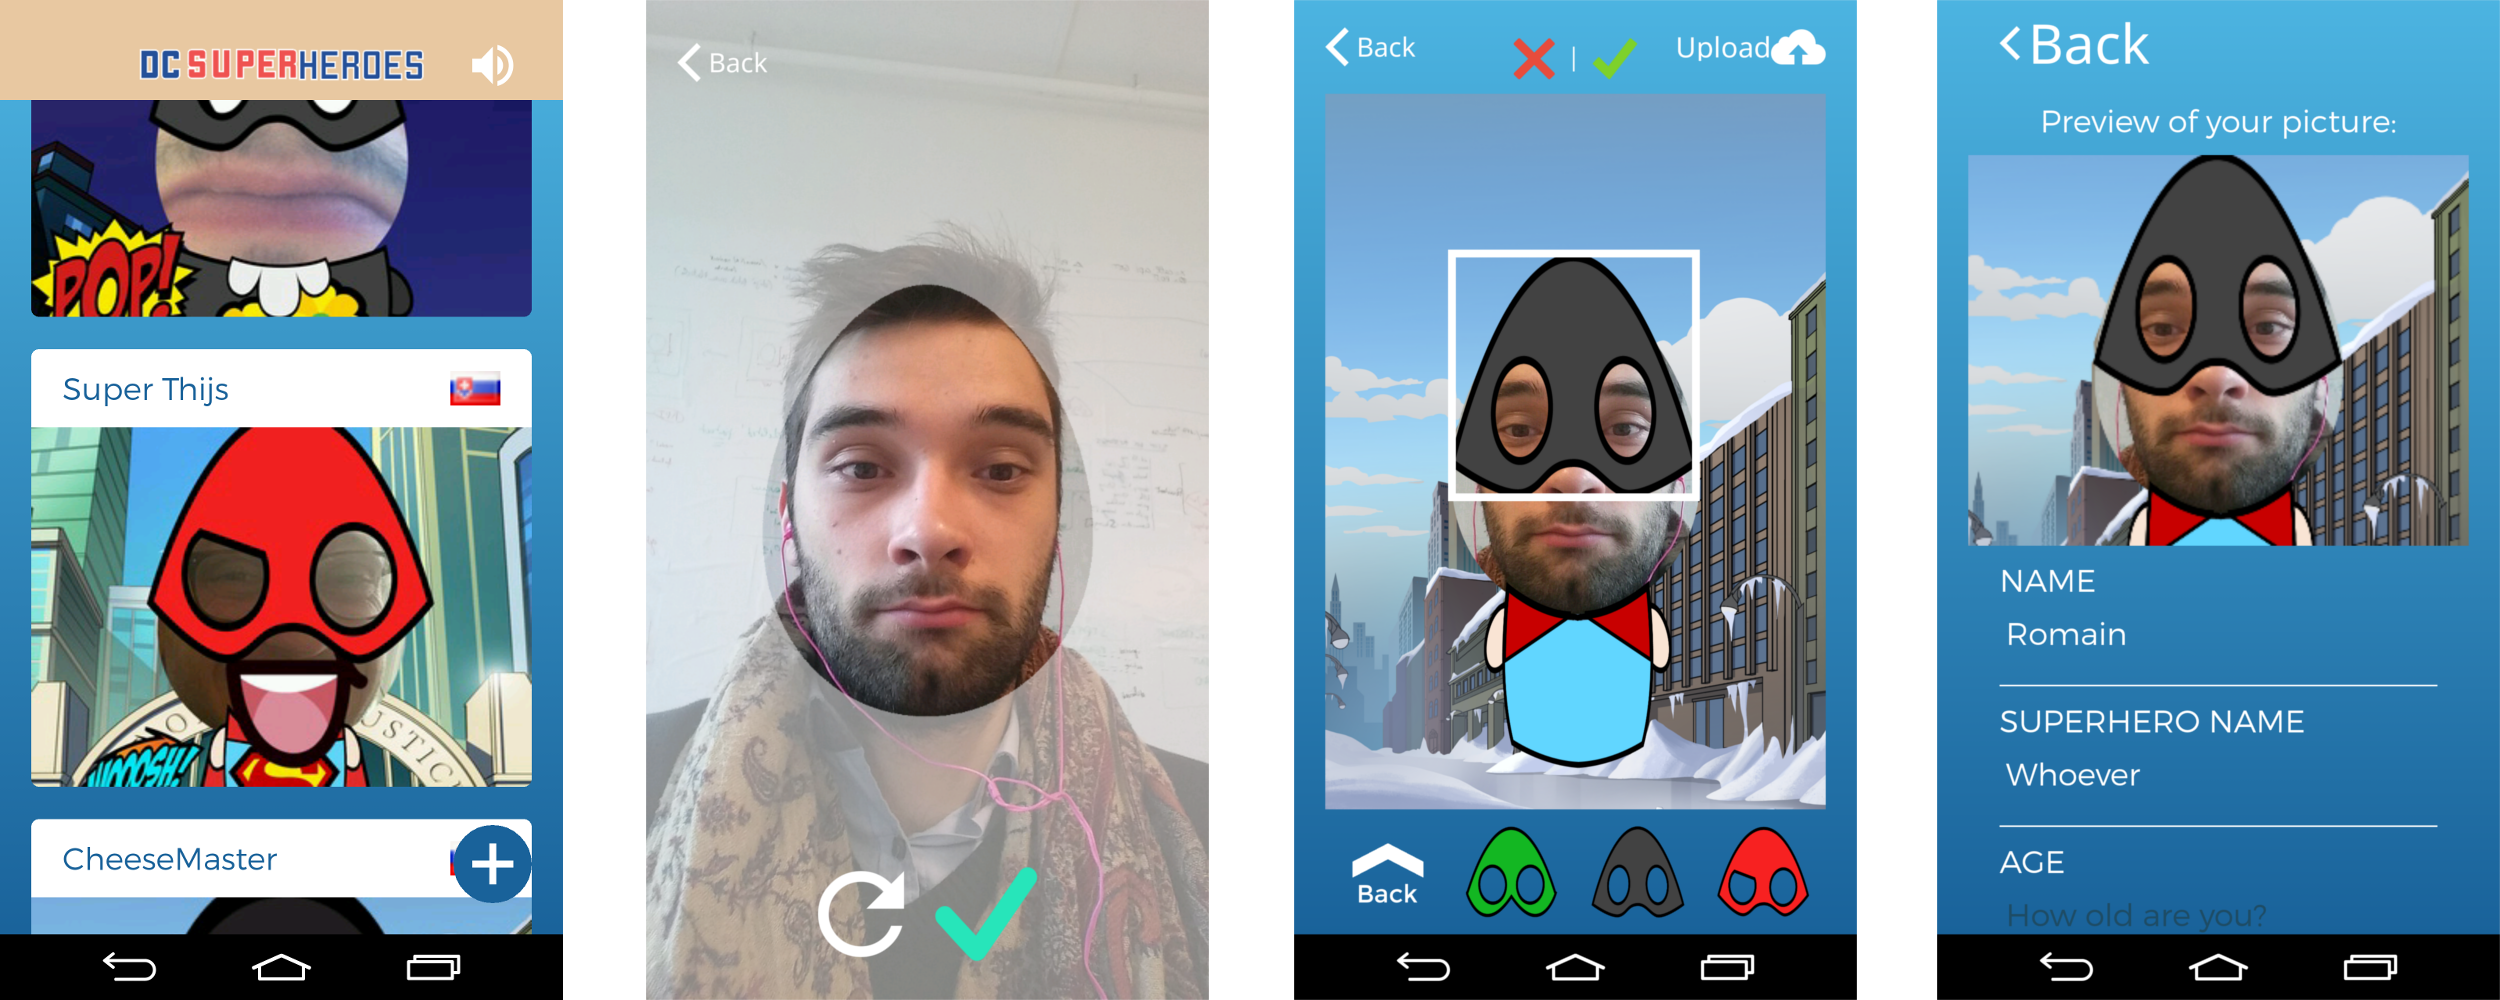
\includegraphics[width=1.00\textwidth]{images/tesco-screens.png}
   \caption[The different pages of the app DC Comics]{From left to right: Feed of pictures, Taking a selfie, Editing the selfie, Uploading it}
\end{figure}

From a technical point of view, the most challenging part was definitively being able to reproduce native capabilities with Titanium, here \textit{drag-and-drop} and \textit{pinch-to-zoom} (used while editing the selfie, third screenshot from left). Matthias took care of this. As for me, I was in charge of the selfie itself (second screenshot). I re-used a widget developed by Nguyen\footnote{\href{https://github.com/TheSmiths-Widgets/ts.camera}{github.com/TheSmiths-Widgets/ts.camera}} (our remote Vietnamese developer). Under the hood, his widget is using two Titanium modules (one for Android and another one for iOS), bringing camera support. His widget acts more as a bridge for our app, adding another layer of abstraction of top of the two modules. However, I had to tweak it a bit to fit at best our requirements. We needed it to be highly flexible regarding positioning and sizing, as the Android ecosystem includes tons of different screens. Pierre was responsible for the upload (last screenshot).

\medskip

After struggling a bit with layouts, I eventually came up with something working. I jumped onto another part of the project, the login page, which was pretty easy to develop. Two text inputs, a call to our REST API, and finally giving some feedback to the user. I forgot to mention, but with this project once again, we decided to go with \href{http://www.parse.com/}{www.parse.com}. We did not even develop our own API, we simply used the one provided natively by Parse to access and manipulate classes\footnote{\href{https://parse.com/docs/rest/guide}{parse.com/docs/rest/guide}}.

\subsection{Managing the screens flow}

Near the end of the project, after reviewing the app, I got assigned the screen flow. The way the end-user would go from one screen to another one, stacking the screens, closing them at the right time. The solution I decided to implement meets a logical flow, quite natural to users.

\begin{enumerate}
  \item From the feed, the users can start creating a new picture, by pressing a button. A new screen with the camera embedded appears.
  \item They can take a selfie and re-try as many times as they want (thanks to a button). When satisfied with the selfie, the editor is launched by pressing another button. The selfie screen is added to a stack of controllers to be closed.
  \item From the editor, users can go back to the selfie screen by pressing "Back" on top of the screen, or the Android-specific back button.
  \item When done with editing, the upload screen appears and the editor is added to the stack (which now contains two controllers).
  \item Here again, users can go back to the editor screen by pressing "Back" on top of the screen, or the Android-specific back button.
  \item The user now fills few input texts and uploads the picture. At the end of the upload, the user can either go back to the feed or take another picture. The current controller (upload) adds itself to the stack of controllers. Then it opens the selfie controller if needed. Eventually, it closes each controller from the stack, one by one (including itself).
  \item When the user goes back to the feed (if they chose to do so), the feed refreshes itself (thanks to an event triggered, '\lstinline{focus}', which fundamentally means that the controller just acquired the focus back).
\end{enumerate}

The following piece of code shows how a controller adds itself to the list of controllers to be closed.

\lstset{
    numbers=left
}
\javascript
\begin{lstlisting}
const args = arguments[0]; // arguments received from another controller at launch

...

// Launching another controller, here the editor starts the upload controller
Alloy.createController('upload', {
    picture: picture,
    toBeClosed: [$.container].concat(args && args.toBeClosed ? args.toBeClosed : [])
})
\end{lstlisting}
\lstset{
    numbers=none
}

The line 8 shows exactly how the controller adds itself (\lstinline{$.container}) to the already existing stack (array actually, the order does not matter) of controllers. As one can see, it also passes that stack to the next controller.\\
Below is how the final controller closes them all and redirects the user to either the feed or the selfie screen:

\begin{lstlisting}
if (e.goto == null || e.goto !== 'feed') {
    Alloy.createController('selfie');
}
[$.container].concat(args && args.toBeClosed ? args.toBeClosed : []).forEach(function(container) {
    if (container != null) {
        container.close();
    }
});
\end{lstlisting}
This controller management is pretty simple but yet works as expected.

\section{Conclusion}

We met the deadline. As I am writing theses lines (January, \nth{22}), we just finished the app. We are now waiting for accesses to the stores (Android and Apple), should we receive them anytime soon from our client.

\medskip

This project did put us under pressure, mostly because of the tight schedule. Manipulating graphical elements was very challenging as well. Every time Matthias would fix the editor, we would detect weird bugs, not to mention the huge differences between Android and iOS.

At last, we made it. We are pretty proud of the final product, and had a lot of fun developing it. I must admit that the app itself is really amusing and we hope the employees will enjoy it as much as we did.

\medskip

Regarding the technical aspects, we used the same tools as with our previous projects, nothing new. We faced big problems with Titanium, mainly due to a lack of consistency across platforms (Android and iOS). Sometimes, the app would not behave the same way, on different platforms, which convinced me cross-platform is not well suited for such specific projects. It rather fits simple projects that do not involve complex UI stuff. Camera management was kind of harsh as well.
\chapter{Conclusion}

This 6-month internship has been extremely rich and intense. I went from being a very beginner at JavaScript to having a quite good knowledge of it. I made big use of ECMAScript 2015 (or ES6), the last official release of the JavaScript specifications (the standard most JavaScript engines tend to implement). It gave me enough insights to measure efficiently the pros and cons of Object-Oriented Programming compared to Prototype-Based Programming (JavaScript supports both paradigms, although it was historically Prototype-Based).\\
At some point, I did some Functional Programming thanks to JavaScript libraries (and Matthias' willingness), not for a long time, but long enough to inspire me and aroused my curiosity (even though I had already used Haskell in the past). I am pretty sure that I will dig into it any time soon. JavaScript truly is an extremely powerful language, too often misunderstood and disregarded (just like PHP is). It used to be very messy but now, more and more, ECMAScript tries to fix problems and break down misconceptions. JavaScript offers developers a lot of freedom, it is just up to them to keep consistent and avoid common and too well known pitfalls. This freedom is the true strength of JavaScript. Bringing Object-Oriented stuff in the latest specifications is just syntactic sugar. In the meantime, they also added, in ES5 and ES6, features from the functional world, like \lstinline{map}, \lstinline{reduce}, or Promises (although this one is a moot point), which is, in my opinion, really awesome.\\
To briefly conclude about JavaScript, I honestly enjoyed working with this language. It is one of the most powerful languages in the world. It is getting incredibly trendy right now. Everyday there is a new revolutionary framework or library coming out (React and Cycle.js are probably the best examples, not to mention architectures like Facebook's Flux and Relay or the awesome Redux). React programming is the new hotness, thanks to JavaScript. JavaScript's future is, with no doubt, bright.

\bigskip

There is a lot to say about cross-platform development, especially on mobile platforms. I was really doubtful when I first saw the internship offer. I had heard lots of bad things about this, in general. Overall, feedback was pretty bad. So I thought "let's give it a try, do not think about what you heard, take a fresh approach".\\
During the first few weeks, I was somehow amazed by the power of Titanium. It supported most of the features of Android and iOS, and more importantly, it was based on JavaScript. One codebase to rule them all. Then, little by little, came the disillusionment. Obsolete and outdated documentation, bad support of the latest features. I remember when Android Marshmallow was publicly released for general availability (October 2015), we had had to wait a few weeks, solely to be able to compile and run apps on it. Furthermore, there is a growing lack of features, especially those brought by the Google Play Services. I am not confident with iOS so I can not actually tell, but according to my colleagues it is as miserable. Sometimes, we would expect a specific behavior from a piece of code, and it would have a completely different effect from a platform to the other.\\
As I said earlier in this report, cross-platform development, or at least Titanium, is well suited for simple apps with commonly encountered features. There is definitely a comfort zone with Titanium and you do not want to get out of it, at all.\\
Recently, in January 2016, Appcelerator has been acquired by another company. At the Smiths, we saw it as a bad sign given to the community. We foreshadowed a dark future for Titanium. On the opposite world of React-native (based on React), the growing community and the support of Facebook is way more reassuring.\\
For the time being, I am still not convinced at all. Instead of cross-platform solutions, I would rather go with native development (Java or Objective-C/Swift). Anyway, I do not truly believe in mobile apps in the long run...

\bigskip

A third aspect of this internship is obviously the fact that it was a startup. Despite it was my second significant experience in a startup, this one was rather different as The Smiths is an agency. As part of a small team, I was directly exposed to most aspects of the startup life. Besides The Smiths, as I was working in an incubator having dozens of startups, from the big ones employing many people and occupying whole floors to the very small ones (less than five people, sometimes only a founder), I have had the chance to talk to many other people. Some of them would sometimes tell me their stories. I am aware of the Silicon Valley Cult\footnote{\href{https://thinkfaster.co/2015/12/beware-of-the-silicon-valley-cult/}{thinkfaster.co/2015/12/beware-of-the-silicon-valley-cult}} and thus am extremely cautious when dealing with startup offers but I definitely have no regret with that one. The Smiths were unlikely to fail as it was an agency, not a startup selling its own product or service. Being daily among startups was awesome as it taught me a lot. I envision a bright future for many of them. Founding a company some day after graduation has always been on my mind. Now, I have a better understanding of the long way it is.

\bigskip

From a personal point a view, I have bigger dreams. I do not want to work on meaningless projects. I do not believe in the mobile industry. I only see it as entertainment. I am not getting my hopes up about it, I am fairly down-to-Earth; I honestly believe the era of mobile is on its descending slope. I just want to do something that matters -- a bit. Working in an agency for clients means handing them over the project at the end of the contract. There is no point in it for me.\\
Consequently, I will keep on exploring new areas and learning (an engineer, especially a software engineer, never stops learning). Functional programming is something I want to deeply explore. It has been leveraging the entire industry for years (JavaScript is getting more and more functional, Elm is a functional programming language that produces JavaScript, and so on). Most of all, I do not want to be stuck in any particular paradigm nor language. Henceforth, I will try to study many languages, keep an eye on react programming and obviously continue with JavaScript for a bit. Continuous Integration is something I wish was more widely spread, it is definitely a best practice in the \nth{21} century. Testing as well, should be more prominent. Computer Science is still very recent and yet already old. Things are going insanely fast and it is almost always impossible to catch up. I am constantly reshaping what I really want to do -- it might never end -- but it is getting more and more clear to me.


%%%%%%%%% GLOSSARY AND INDEX ON THE SAME PAGE %%%%%%%%%
%\glsaddall % next line will print all entries, not just the ones your mark in your text
%\printglossary[title=Glossary and Index]


%%%%%%%%% BIBLIOGRAPHY %%%%%%%%%
\chapter*{Bibliography}
\markboth{}{\MakeUppercase{Bibliography}}
\addcontentsline{toc}{chapter}{Bibliography}
\printbibliography[heading=subbibintoc,type=unpublished,title={Talks}]
\printbibliography[heading=subbibintoc,type=online,title={Blog posts and documentation}] % heading=subbibintoc show the bibliography in the ToC as a section (heading=bibintoc for as chapter)
\printbibliography[heading=subbibintoc,type=book,title={Books}]


\cleardoublepage

%%%%%%%%% APPENDICES %%%%%%%%%
\begin{appendices}
\chapter{Git: branching model}\label{appendix-git}

\begin{figure}[!h]
   \centering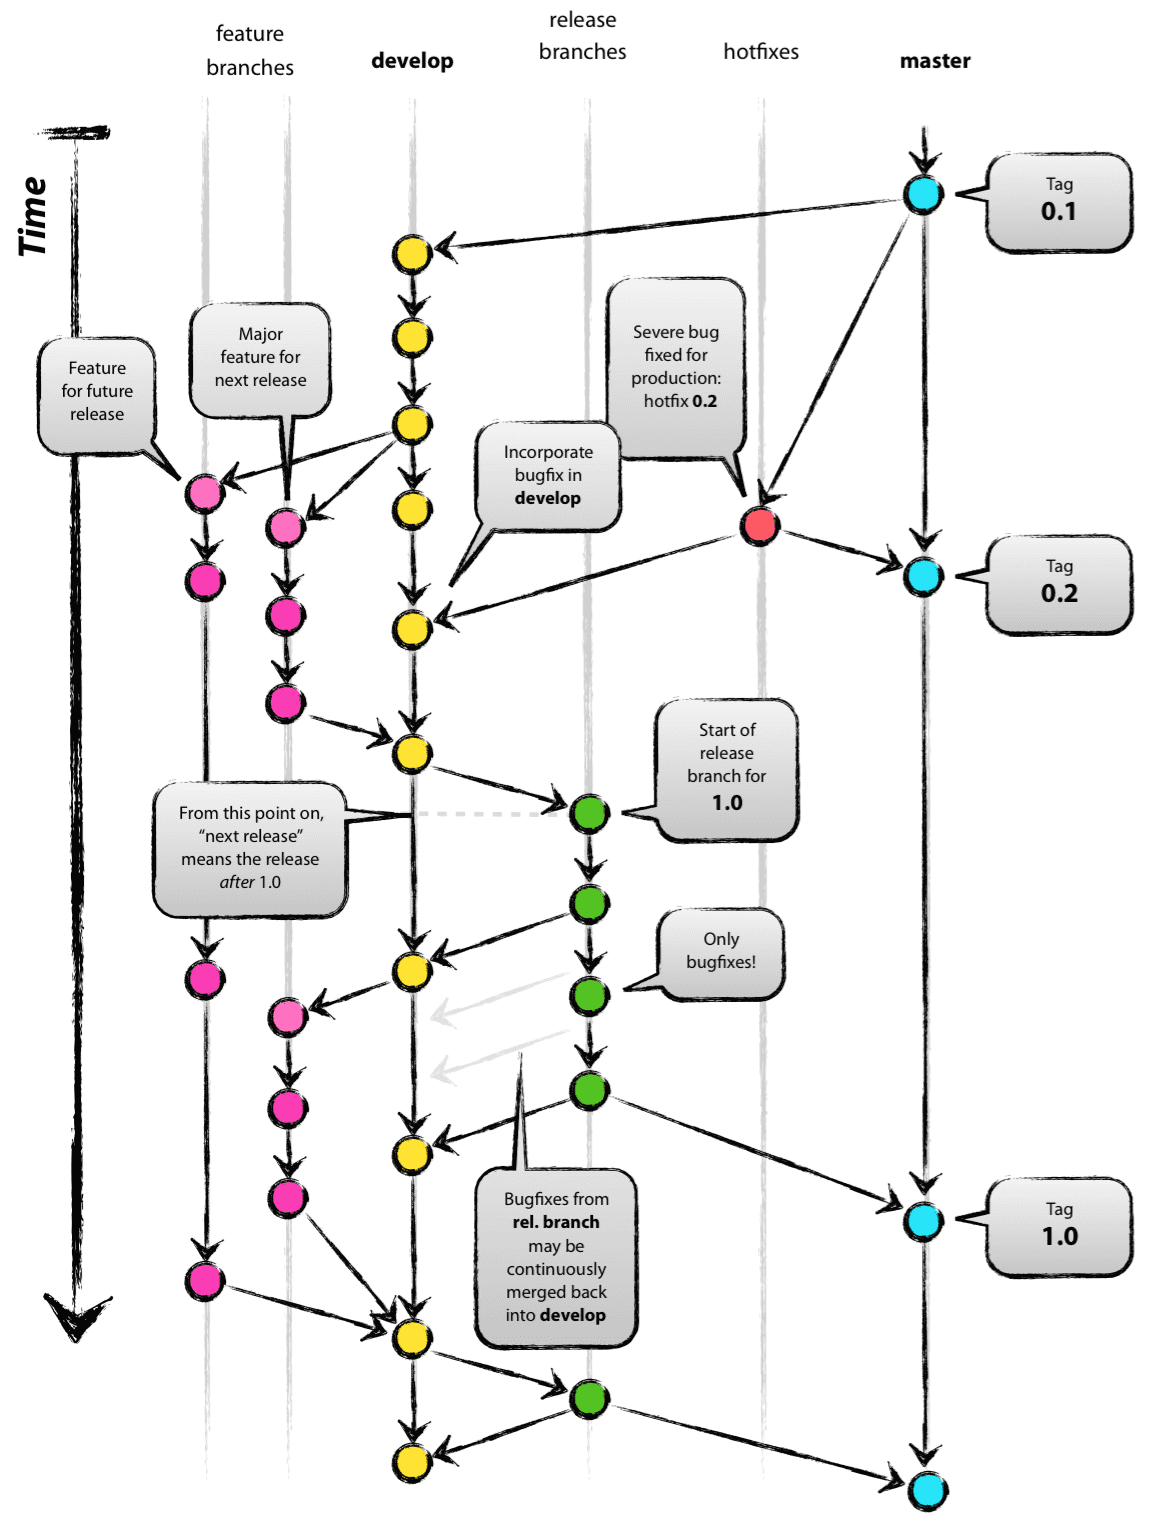
\includegraphics[width=0.92\textwidth]{images/git-branching-model.png}
   \caption[]{Git workflow\\Courtesy of \href{https://twitter.com/nvie/status/644601079985008640}{Vincent Driessen\\Source: \href{http://nvie.com/posts/a-successful-git-branching-model/}{http://nvie.com/posts/a-successful-git-branching-model/}}} % [] allow us to hide that figure from the list of figures
\end{figure}

\chapter{Some of the SQL queries written for Bearleaders}\label{bearleaders-sql}

\sql
\begin{lstlisting}
-- Only the last pictures for each user
SELECT
    filename,
    first.user_id as user
FROM
    profile_photo as first
INNER JOIN
    (select user_id, max(id) as last from profile_photo group by user_id) as second
ON
    first.user_id = second.user_id
    AND first.id = second.last;
\end{lstlisting}
\begin{lstlisting}
-- Get the bearleaders (people who added more than 3 spots)
SELECT
    front_users.id,
    pro.firstname as first_name,
    pro.lastname as last_name,
    front_users.username as username,
    front_users.email as email,
    password,
    website,
    concat(job,if((job is not null and job <> "") and (motto is not null and motto <> ""),\'\n\',\'\'),motto) as biography,
    city as coming_from,
    job,
    "" as linkedin_url
FROM
    front_users, yellow_pages yp, profile pro
WHERE
    password IS NOT NULL AND password <> ""
    AND front_users.id = yp.ypCreator and front_users.id = pro.user_id
    AND email LIKE "%_@__%.__%"
    AND EXISTS (select * from profile_photo where user_id = front_users.id)
    AND firstname IS NOT NULL and firstname <> ""
    AND lastname IS NOT NULL and (lastname <> "" or username = "Concierge")
GROUP BY email
HAVING count(*) > 3;
\end{lstlisting}
\begin{lstlisting}
-- Gettings all the spots
SELECT
    yp_CatID, ypID, "true" as public, FU.email as creator, ypName as name, ypText as description, ypAddress as address, ypURL as website, ypPhone as phone_number, ypLat, ypLng, ypCountry as country, ypPlaats as city, ypMail as email
FROM
    yellow_pages
INNER JOIN
    BEARLEADERS as FU
ON
    ypCreator = FU.id
WHERE
    yp_CatID IS NOT NULL and yp_CatID <> ""
    and ypLat IS NOT NULL
    and ypLng IS NOT NULL
    and ypLogo IS NOT NULL and ypLogo <> ""
    and ref_id = 0
    and ypCountry IS NOT NULL and ypCountry <> ""
    and ypText IS NOT NULL and ypText <> ""
    and ypName IS NOT NULL and ypName <> ""
    and ypAddress IS NOT NULL and ypAddress <> ""
    and ypPlaats IS NOT NULL and ypPlaats <> "";
\end{lstlisting}
\end{appendices}


\end{document}